\documentclass[twoside]{book}

% Packages required by doxygen
\usepackage{fixltx2e}
\usepackage{calc}
\usepackage{doxygen}
\usepackage[export]{adjustbox} % also loads graphicx
\usepackage{graphicx}
\usepackage[utf8]{inputenc}
\usepackage{makeidx}
\usepackage{multicol}
\usepackage{multirow}
\PassOptionsToPackage{warn}{textcomp}
\usepackage{textcomp}
\usepackage[nointegrals]{wasysym}
\usepackage[table]{xcolor}

% Font selection
\usepackage[T1]{fontenc}
\usepackage[scaled=.90]{helvet}
\usepackage{courier}
\usepackage{amssymb}
\usepackage{sectsty}
\renewcommand{\familydefault}{\sfdefault}
\allsectionsfont{%
  \fontseries{bc}\selectfont%
  \color{darkgray}%
}
\renewcommand{\DoxyLabelFont}{%
  \fontseries{bc}\selectfont%
  \color{darkgray}%
}
\newcommand{\+}{\discretionary{\mbox{\scriptsize$\hookleftarrow$}}{}{}}

% Page & text layout
\usepackage{geometry}
\geometry{%
  a4paper,%
  top=2.5cm,%
  bottom=2.5cm,%
  left=2.5cm,%
  right=2.5cm%
}
\tolerance=750
\hfuzz=15pt
\hbadness=750
\setlength{\emergencystretch}{15pt}
\setlength{\parindent}{0cm}
\setlength{\parskip}{0.2cm}
\makeatletter
\renewcommand{\paragraph}{%
  \@startsection{paragraph}{4}{0ex}{-1.0ex}{1.0ex}{%
    \normalfont\normalsize\bfseries\SS@parafont%
  }%
}
\renewcommand{\subparagraph}{%
  \@startsection{subparagraph}{5}{0ex}{-1.0ex}{1.0ex}{%
    \normalfont\normalsize\bfseries\SS@subparafont%
  }%
}
\makeatother

% Headers & footers
\usepackage{fancyhdr}
\pagestyle{fancyplain}
\fancyhead[LE]{\fancyplain{}{\bfseries\thepage}}
\fancyhead[CE]{\fancyplain{}{}}
\fancyhead[RE]{\fancyplain{}{\bfseries\leftmark}}
\fancyhead[LO]{\fancyplain{}{\bfseries\rightmark}}
\fancyhead[CO]{\fancyplain{}{}}
\fancyhead[RO]{\fancyplain{}{\bfseries\thepage}}
\fancyfoot[LE]{\fancyplain{}{}}
\fancyfoot[CE]{\fancyplain{}{}}
\fancyfoot[RE]{\fancyplain{}{\bfseries\scriptsize Generated on Thu Feb 19 2015 15\+:36\+:15 for Chess by Doxygen }}
\fancyfoot[LO]{\fancyplain{}{\bfseries\scriptsize Generated on Thu Feb 19 2015 15\+:36\+:15 for Chess by Doxygen }}
\fancyfoot[CO]{\fancyplain{}{}}
\fancyfoot[RO]{\fancyplain{}{}}
\renewcommand{\footrulewidth}{0.4pt}
\renewcommand{\chaptermark}[1]{%
  \markboth{#1}{}%
}
\renewcommand{\sectionmark}[1]{%
  \markright{\thesection\ #1}%
}

% Indices & bibliography
\usepackage{natbib}
\usepackage[titles]{tocloft}
\setcounter{tocdepth}{3}
\setcounter{secnumdepth}{5}
\makeindex

% Hyperlinks (required, but should be loaded last)
\usepackage{ifpdf}
\ifpdf
  \usepackage[pdftex,pagebackref=true]{hyperref}
\else
  \usepackage[ps2pdf,pagebackref=true]{hyperref}
\fi
\hypersetup{%
  colorlinks=true,%
  linkcolor=blue,%
  citecolor=blue,%
  unicode%
}

% Custom commands
\newcommand{\clearemptydoublepage}{%
  \newpage{\pagestyle{empty}\cleardoublepage}%
}


%===== C O N T E N T S =====

\begin{document}

% Titlepage & ToC
\hypersetup{pageanchor=false,
             bookmarks=true,
             bookmarksnumbered=true,
             pdfencoding=unicode
            }
\pagenumbering{roman}
\begin{titlepage}
\vspace*{7cm}
\begin{center}%
{\Large Chess }\\
\vspace*{1cm}
{\large Generated by Doxygen 1.8.9.1}\\
\vspace*{0.5cm}
{\small Thu Feb 19 2015 15:36:15}\\
\end{center}
\end{titlepage}
\clearemptydoublepage
\tableofcontents
\clearemptydoublepage
\pagenumbering{arabic}
\hypersetup{pageanchor=true}

%--- Begin generated contents ---
\chapter{Hierarchical Index}
\section{Class Hierarchy}
This inheritance list is sorted roughly, but not completely, alphabetically\+:\begin{DoxyCompactList}
\item \contentsline{section}{Bishop\+Test}{\pageref{class_bishop_test}}{}
\item \contentsline{section}{Board}{\pageref{class_board}}{}
\item \contentsline{section}{Board\+Test}{\pageref{class_board_test}}{}
\item \contentsline{section}{Game}{\pageref{class_game}}{}
\item \contentsline{section}{Hopper\+Test}{\pageref{class_hopper_test}}{}
\item \contentsline{section}{Juggernaut\+Test}{\pageref{class_juggernaut_test}}{}
\item \contentsline{section}{King\+Test}{\pageref{class_king_test}}{}
\item \contentsline{section}{Knight\+Test}{\pageref{class_knight_test}}{}
\item \contentsline{section}{Pawn\+Test}{\pageref{class_pawn_test}}{}
\item \contentsline{section}{Piece}{\pageref{class_piece}}{}
\begin{DoxyCompactList}
\item \contentsline{section}{Bishop}{\pageref{class_bishop}}{}
\item \contentsline{section}{Hopper}{\pageref{class_hopper}}{}
\item \contentsline{section}{Juggernaut}{\pageref{class_juggernaut}}{}
\item \contentsline{section}{King}{\pageref{class_king}}{}
\item \contentsline{section}{Knight}{\pageref{class_knight}}{}
\item \contentsline{section}{Pawn}{\pageref{class_pawn}}{}
\item \contentsline{section}{Queen}{\pageref{class_queen}}{}
\item \contentsline{section}{Rook}{\pageref{class_rook}}{}
\end{DoxyCompactList}
\item \contentsline{section}{Player}{\pageref{class_player}}{}
\item \contentsline{section}{Queen\+Test}{\pageref{class_queen_test}}{}
\item \contentsline{section}{Rook\+Test}{\pageref{class_rook_test}}{}
\item J\+Frame\begin{DoxyCompactList}
\item \contentsline{section}{Board\+Layout}{\pageref{class_board_layout}}{}
\end{DoxyCompactList}
\item J\+Label\begin{DoxyCompactList}
\item \contentsline{section}{Chess\+Label}{\pageref{class_chess_label}}{}
\end{DoxyCompactList}
\end{DoxyCompactList}

\chapter{Class Index}
\section{Class List}
Here are the classes, structs, unions and interfaces with brief descriptions\+:\begin{DoxyCompactList}
\item\contentsline{section}{\hyperlink{class_bishop}{Bishop} }{\pageref{class_bishop}}{}
\item\contentsline{section}{\hyperlink{class_bishop_test}{Bishop\+Test} }{\pageref{class_bishop_test}}{}
\item\contentsline{section}{\hyperlink{class_board}{Board} }{\pageref{class_board}}{}
\item\contentsline{section}{\hyperlink{class_board_layout}{Board\+Layout} }{\pageref{class_board_layout}}{}
\item\contentsline{section}{\hyperlink{class_board_test}{Board\+Test} }{\pageref{class_board_test}}{}
\item\contentsline{section}{\hyperlink{class_chess_label}{Chess\+Label} }{\pageref{class_chess_label}}{}
\item\contentsline{section}{\hyperlink{class_game}{Game} }{\pageref{class_game}}{}
\item\contentsline{section}{\hyperlink{class_hopper}{Hopper} }{\pageref{class_hopper}}{}
\item\contentsline{section}{\hyperlink{class_hopper_test}{Hopper\+Test} }{\pageref{class_hopper_test}}{}
\item\contentsline{section}{\hyperlink{class_juggernaut}{Juggernaut} }{\pageref{class_juggernaut}}{}
\item\contentsline{section}{\hyperlink{class_juggernaut_test}{Juggernaut\+Test} }{\pageref{class_juggernaut_test}}{}
\item\contentsline{section}{\hyperlink{class_king}{King} }{\pageref{class_king}}{}
\item\contentsline{section}{\hyperlink{class_king_test}{King\+Test} }{\pageref{class_king_test}}{}
\item\contentsline{section}{\hyperlink{class_knight}{Knight} }{\pageref{class_knight}}{}
\item\contentsline{section}{\hyperlink{class_knight_test}{Knight\+Test} }{\pageref{class_knight_test}}{}
\item\contentsline{section}{\hyperlink{class_pawn}{Pawn} }{\pageref{class_pawn}}{}
\item\contentsline{section}{\hyperlink{class_pawn_test}{Pawn\+Test} }{\pageref{class_pawn_test}}{}
\item\contentsline{section}{\hyperlink{class_piece}{Piece} }{\pageref{class_piece}}{}
\item\contentsline{section}{\hyperlink{class_player}{Player} }{\pageref{class_player}}{}
\item\contentsline{section}{\hyperlink{class_queen}{Queen} }{\pageref{class_queen}}{}
\item\contentsline{section}{\hyperlink{class_queen_test}{Queen\+Test} }{\pageref{class_queen_test}}{}
\item\contentsline{section}{\hyperlink{class_rook}{Rook} }{\pageref{class_rook}}{}
\item\contentsline{section}{\hyperlink{class_rook_test}{Rook\+Test} }{\pageref{class_rook_test}}{}
\end{DoxyCompactList}

\chapter{Class Documentation}
\hypertarget{class_bishop}{}\section{Bishop Class Reference}
\label{class_bishop}\index{Bishop@{Bishop}}
Inheritance diagram for Bishop\+:\begin{figure}[H]
\begin{center}
\leavevmode
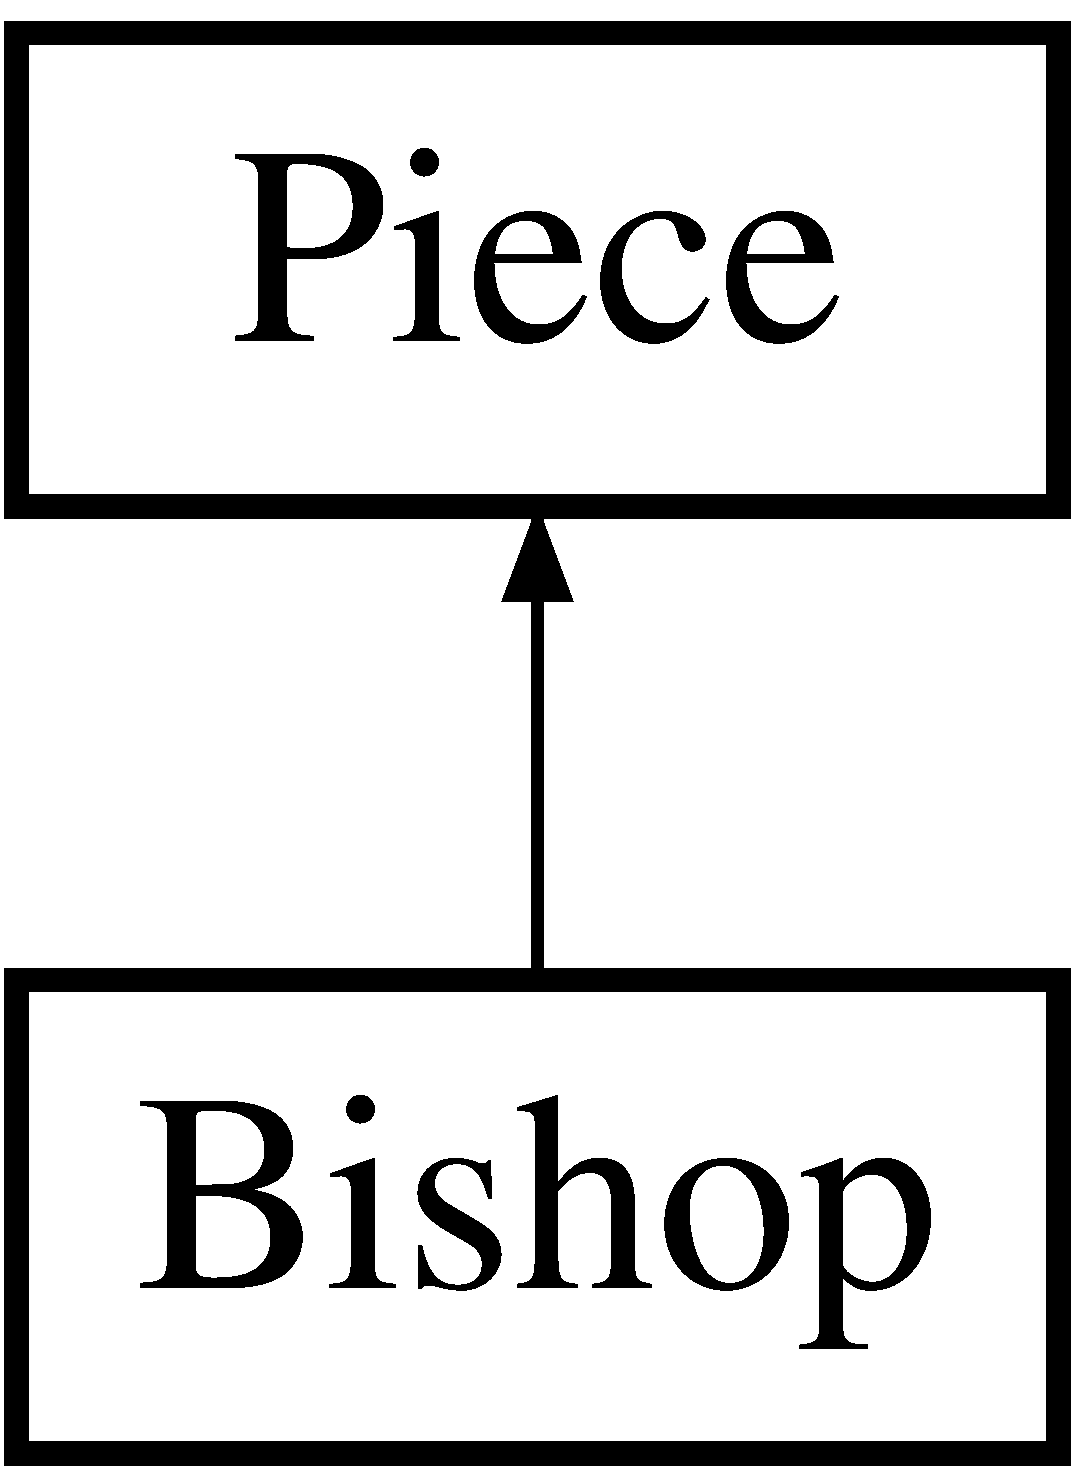
\includegraphics[height=2.000000cm]{class_bishop}
\end{center}
\end{figure}
\subsection*{Public Member Functions}
\begin{DoxyCompactItemize}
\item 
\hyperlink{class_bishop_a7789264cbdc50734a376431858ab391e}{Bishop} (boolean color, int x\+Coord, int y\+Coord)
\item 
boolean \hyperlink{class_bishop_a3977c5c6233c9613b74261136e29eeb5}{is\+Valid\+Move} (\hyperlink{class_board}{Board} board, int to\+X, int to\+Y)
\item 
boolean \hyperlink{class_bishop_af843be483752642ab77dc6741c8d0a14}{piece\+In\+Way\+Diagonal} (\hyperlink{class_board}{Board} board, int to\+X, int to\+Y)
\end{DoxyCompactItemize}
\subsection*{Additional Inherited Members}


\subsection{Constructor \& Destructor Documentation}
\hypertarget{class_bishop_a7789264cbdc50734a376431858ab391e}{}\index{Bishop@{Bishop}!Bishop@{Bishop}}
\index{Bishop@{Bishop}!Bishop@{Bishop}}
\subsubsection[{Bishop}]{\setlength{\rightskip}{0pt plus 5cm}Bishop.\+Bishop (
\begin{DoxyParamCaption}
\item[{boolean}]{color, }
\item[{int}]{x\+Coord, }
\item[{int}]{y\+Coord}
\end{DoxyParamCaption}
)}\label{class_bishop_a7789264cbdc50734a376431858ab391e}
\hyperlink{class_bishop}{Bishop} Constructor 
\begin{DoxyParams}{Parameters}
{\em color} & \\
\hline
{\em x\+Coord} & \\
\hline
{\em y\+Coord} & \\
\hline
\end{DoxyParams}


\subsection{Member Function Documentation}
\hypertarget{class_bishop_a3977c5c6233c9613b74261136e29eeb5}{}\index{Bishop@{Bishop}!is\+Valid\+Move@{is\+Valid\+Move}}
\index{is\+Valid\+Move@{is\+Valid\+Move}!Bishop@{Bishop}}
\subsubsection[{is\+Valid\+Move}]{\setlength{\rightskip}{0pt plus 5cm}boolean Bishop.\+is\+Valid\+Move (
\begin{DoxyParamCaption}
\item[{{\bf Board}}]{board, }
\item[{int}]{to\+X, }
\item[{int}]{to\+Y}
\end{DoxyParamCaption}
)}\label{class_bishop_a3977c5c6233c9613b74261136e29eeb5}
Check if Valid Move 
\begin{DoxyParams}{Parameters}
{\em board} & \\
\hline
{\em to\+X} & \\
\hline
{\em to\+Y} & \\
\hline
\end{DoxyParams}
\begin{DoxyReturn}{Returns}

\end{DoxyReturn}
\hypertarget{class_bishop_af843be483752642ab77dc6741c8d0a14}{}\index{Bishop@{Bishop}!piece\+In\+Way\+Diagonal@{piece\+In\+Way\+Diagonal}}
\index{piece\+In\+Way\+Diagonal@{piece\+In\+Way\+Diagonal}!Bishop@{Bishop}}
\subsubsection[{piece\+In\+Way\+Diagonal}]{\setlength{\rightskip}{0pt plus 5cm}boolean Bishop.\+piece\+In\+Way\+Diagonal (
\begin{DoxyParamCaption}
\item[{{\bf Board}}]{board, }
\item[{int}]{to\+X, }
\item[{int}]{to\+Y}
\end{DoxyParamCaption}
)}\label{class_bishop_af843be483752642ab77dc6741c8d0a14}
Check if collision along diagonal path 
\begin{DoxyParams}{Parameters}
{\em board} & \\
\hline
{\em to\+X} & \\
\hline
{\em to\+Y} & \\
\hline
\end{DoxyParams}
\begin{DoxyReturn}{Returns}

\end{DoxyReturn}


The documentation for this class was generated from the following file\+:\begin{DoxyCompactItemize}
\item 
src/Bishop.\+java\end{DoxyCompactItemize}

\hypertarget{class_bishop_test}{}\section{Bishop\+Test Class Reference}
\label{class_bishop_test}\index{Bishop\+Test@{Bishop\+Test}}
\subsection*{Public Member Functions}
\begin{DoxyCompactItemize}
\item 
\hypertarget{class_bishop_test_a7028c52f8952b85a212e94413377dd1d}{}void {\bfseries test\+Simple\+Move} ()  throws Exception \label{class_bishop_test_a7028c52f8952b85a212e94413377dd1d}

\item 
\hypertarget{class_bishop_test_abbec6ec95aa8fb463dc3509d2ee5c4af}{}void {\bfseries test\+Capture} ()  throws Exception \label{class_bishop_test_abbec6ec95aa8fb463dc3509d2ee5c4af}

\item 
\hypertarget{class_bishop_test_acc47e5046fcdfc06da3a36505cc02857}{}void {\bfseries test\+Piece\+In\+Way} ()  throws Exception \label{class_bishop_test_acc47e5046fcdfc06da3a36505cc02857}

\item 
\hypertarget{class_bishop_test_ab3de9c5e3de068dfb4c82a5d27bdd61e}{}void {\bfseries test\+Illegal\+Move} ()  throws Exception \label{class_bishop_test_ab3de9c5e3de068dfb4c82a5d27bdd61e}

\end{DoxyCompactItemize}


The documentation for this class was generated from the following file\+:\begin{DoxyCompactItemize}
\item 
Test/Bishop\+Test.\+java\end{DoxyCompactItemize}

\hypertarget{class_board}{}\section{Board Class Reference}
\label{class_board}\index{Board@{Board}}
\subsection*{Public Member Functions}
\begin{DoxyCompactItemize}
\item 
int \hyperlink{class_board_a514e9e5c80174d567fe5f1311b105a24}{get\+Width} ()
\item 
int \hyperlink{class_board_a89073052a738d3960b573a695e1aafed}{get\+Height} ()
\item 
void \hyperlink{class_board_a7860357debff0df2cad62b14305e7a99}{set\+Width} (int width)
\item 
void \hyperlink{class_board_a4690b660f6edd459c4f02f77dc551478}{set\+Height} (int height)
\item 
\hyperlink{class_piece}{Piece} \hyperlink{class_board_ad4228992ab9ea75d6e36546047971ace}{get\+Piece} (int x\+Coord, int y\+Coord)
\item 
void \hyperlink{class_board_a71ea4447e55dc3b152d5b5d3ea47fc9a}{set\+Piece} (\hyperlink{class_piece}{Piece} new\+Piece, int x\+Coord, int y\+Coord)
\item 
boolean \hyperlink{class_board_a4b0170c56fbe6bc4cea24d53c9666c5f}{check\+Piece\+On\+Board} (int x\+Coord, int y\+Coord)
\item 
void \hyperlink{class_board_abd1044868608621ab830d8e2dfaaf799}{remove\+Piece} (int x\+Coord, int y\+Coord)
\item 
\hypertarget{class_board_aea5a90bdae0d9b4c25441cc08bc2ac64}{}void {\bfseries replace\+Piece} (int to\+X, int to\+Y, \hyperlink{class_piece}{Piece} piece)\label{class_board_aea5a90bdae0d9b4c25441cc08bc2ac64}

\end{DoxyCompactItemize}
\subsection*{Protected Attributes}
\begin{DoxyCompactItemize}
\item 
\hypertarget{class_board_a2f9e52c8f83e21be433bb3a323834595}{}int {\bfseries width}\label{class_board_a2f9e52c8f83e21be433bb3a323834595}

\item 
\hypertarget{class_board_adbbf79735f96938460ee9bd4056ced62}{}int {\bfseries height}\label{class_board_adbbf79735f96938460ee9bd4056ced62}

\item 
\hypertarget{class_board_aa29961b0c52a6744018ff6060bd3c116}{}\hyperlink{class_piece}{Piece}\mbox{[}$\,$\mbox{]}\mbox{[}$\,$\mbox{]} {\bfseries piece} = new \hyperlink{class_piece}{Piece}\mbox{[}8\mbox{]}\mbox{[}8\mbox{]}\label{class_board_aa29961b0c52a6744018ff6060bd3c116}

\end{DoxyCompactItemize}


\subsection{Member Function Documentation}
\hypertarget{class_board_a4b0170c56fbe6bc4cea24d53c9666c5f}{}\index{Board@{Board}!check\+Piece\+On\+Board@{check\+Piece\+On\+Board}}
\index{check\+Piece\+On\+Board@{check\+Piece\+On\+Board}!Board@{Board}}
\subsubsection[{check\+Piece\+On\+Board}]{\setlength{\rightskip}{0pt plus 5cm}boolean Board.\+check\+Piece\+On\+Board (
\begin{DoxyParamCaption}
\item[{int}]{x\+Coord, }
\item[{int}]{y\+Coord}
\end{DoxyParamCaption}
)}\label{class_board_a4b0170c56fbe6bc4cea24d53c9666c5f}
Check if a piece exists on board at coordinate


\begin{DoxyParams}{Parameters}
{\em x\+Coord} & \\
\hline
{\em y\+Coord} & \\
\hline
\end{DoxyParams}
\begin{DoxyReturn}{Returns}

\end{DoxyReturn}
\hypertarget{class_board_a89073052a738d3960b573a695e1aafed}{}\index{Board@{Board}!get\+Height@{get\+Height}}
\index{get\+Height@{get\+Height}!Board@{Board}}
\subsubsection[{get\+Height}]{\setlength{\rightskip}{0pt plus 5cm}int Board.\+get\+Height (
\begin{DoxyParamCaption}
{}
\end{DoxyParamCaption}
)}\label{class_board_a89073052a738d3960b573a695e1aafed}
Retrieve the height of the board \begin{DoxyReturn}{Returns}

\end{DoxyReturn}
\hypertarget{class_board_ad4228992ab9ea75d6e36546047971ace}{}\index{Board@{Board}!get\+Piece@{get\+Piece}}
\index{get\+Piece@{get\+Piece}!Board@{Board}}
\subsubsection[{get\+Piece}]{\setlength{\rightskip}{0pt plus 5cm}{\bf Piece} Board.\+get\+Piece (
\begin{DoxyParamCaption}
\item[{int}]{x\+Coord, }
\item[{int}]{y\+Coord}
\end{DoxyParamCaption}
)}\label{class_board_ad4228992ab9ea75d6e36546047971ace}
Return the piece at this coordinate


\begin{DoxyParams}{Parameters}
{\em x\+Coord} & \\
\hline
{\em y\+Coord} & \\
\hline
\end{DoxyParams}
\begin{DoxyReturn}{Returns}

\end{DoxyReturn}
\hypertarget{class_board_a514e9e5c80174d567fe5f1311b105a24}{}\index{Board@{Board}!get\+Width@{get\+Width}}
\index{get\+Width@{get\+Width}!Board@{Board}}
\subsubsection[{get\+Width}]{\setlength{\rightskip}{0pt plus 5cm}int Board.\+get\+Width (
\begin{DoxyParamCaption}
{}
\end{DoxyParamCaption}
)}\label{class_board_a514e9e5c80174d567fe5f1311b105a24}
Retrieve the width of the board \begin{DoxyReturn}{Returns}

\end{DoxyReturn}
\hypertarget{class_board_abd1044868608621ab830d8e2dfaaf799}{}\index{Board@{Board}!remove\+Piece@{remove\+Piece}}
\index{remove\+Piece@{remove\+Piece}!Board@{Board}}
\subsubsection[{remove\+Piece}]{\setlength{\rightskip}{0pt plus 5cm}void Board.\+remove\+Piece (
\begin{DoxyParamCaption}
\item[{int}]{x\+Coord, }
\item[{int}]{y\+Coord}
\end{DoxyParamCaption}
)}\label{class_board_abd1044868608621ab830d8e2dfaaf799}
Set the piece at this X\+Y coordinate to be null


\begin{DoxyParams}{Parameters}
{\em x\+Coord} & \\
\hline
{\em y\+Coord} & \\
\hline
\end{DoxyParams}
\hypertarget{class_board_a4690b660f6edd459c4f02f77dc551478}{}\index{Board@{Board}!set\+Height@{set\+Height}}
\index{set\+Height@{set\+Height}!Board@{Board}}
\subsubsection[{set\+Height}]{\setlength{\rightskip}{0pt plus 5cm}void Board.\+set\+Height (
\begin{DoxyParamCaption}
\item[{int}]{height}
\end{DoxyParamCaption}
)}\label{class_board_a4690b660f6edd459c4f02f77dc551478}
Set the height of the board 
\begin{DoxyParams}{Parameters}
{\em height} & \\
\hline
\end{DoxyParams}
\hypertarget{class_board_a71ea4447e55dc3b152d5b5d3ea47fc9a}{}\index{Board@{Board}!set\+Piece@{set\+Piece}}
\index{set\+Piece@{set\+Piece}!Board@{Board}}
\subsubsection[{set\+Piece}]{\setlength{\rightskip}{0pt plus 5cm}void Board.\+set\+Piece (
\begin{DoxyParamCaption}
\item[{{\bf Piece}}]{new\+Piece, }
\item[{int}]{x\+Coord, }
\item[{int}]{y\+Coord}
\end{DoxyParamCaption}
)}\label{class_board_a71ea4447e55dc3b152d5b5d3ea47fc9a}
Placing a piece on the board at a coordinate


\begin{DoxyParams}{Parameters}
{\em new\+Piece} & \\
\hline
{\em x\+Coord} & \\
\hline
{\em y\+Coord} & \\
\hline
\end{DoxyParams}
\hypertarget{class_board_a7860357debff0df2cad62b14305e7a99}{}\index{Board@{Board}!set\+Width@{set\+Width}}
\index{set\+Width@{set\+Width}!Board@{Board}}
\subsubsection[{set\+Width}]{\setlength{\rightskip}{0pt plus 5cm}void Board.\+set\+Width (
\begin{DoxyParamCaption}
\item[{int}]{width}
\end{DoxyParamCaption}
)}\label{class_board_a7860357debff0df2cad62b14305e7a99}
Set the width of the board 
\begin{DoxyParams}{Parameters}
{\em width} & \\
\hline
\end{DoxyParams}


The documentation for this class was generated from the following file\+:\begin{DoxyCompactItemize}
\item 
src/Board.\+java\end{DoxyCompactItemize}

\hypertarget{class_board_layout}{}\section{Board\+Layout Class Reference}
\label{class_board_layout}\index{Board\+Layout@{Board\+Layout}}
Inheritance diagram for Board\+Layout\+:\begin{figure}[H]
\begin{center}
\leavevmode
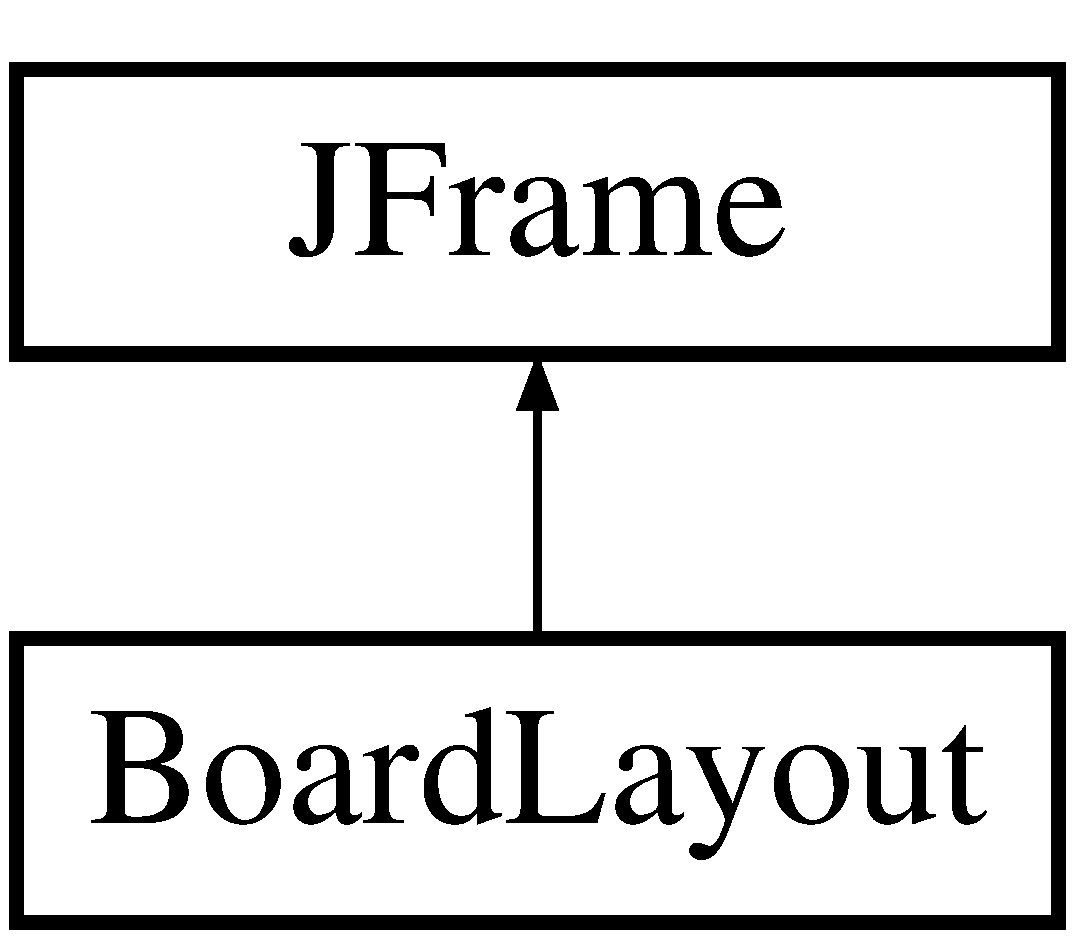
\includegraphics[height=2.000000cm]{class_board_layout}
\end{center}
\end{figure}


The documentation for this class was generated from the following file\+:\begin{DoxyCompactItemize}
\item 
src/Board\+Layout.\+java\end{DoxyCompactItemize}

\hypertarget{class_board_test}{}\section{Board\+Test Class Reference}
\label{class_board_test}\index{Board\+Test@{Board\+Test}}
\subsection*{Public Member Functions}
\begin{DoxyCompactItemize}
\item 
\hypertarget{class_board_test_a664f63b96bc863e0f8f0a5c45744b74d}{}void {\bfseries test\+Get\+Piece} ()  throws Exception \label{class_board_test_a664f63b96bc863e0f8f0a5c45744b74d}

\item 
\hypertarget{class_board_test_adaac6704ceb2345fe9ce1945edc7480a}{}void {\bfseries test\+Check\+Piece\+On\+Board} ()  throws Exception \label{class_board_test_adaac6704ceb2345fe9ce1945edc7480a}

\end{DoxyCompactItemize}


The documentation for this class was generated from the following file\+:\begin{DoxyCompactItemize}
\item 
Test/Board\+Test.\+java\end{DoxyCompactItemize}

\hypertarget{class_chess_label}{}\section{Chess\+Label Class Reference}
\label{class_chess_label}\index{Chess\+Label@{Chess\+Label}}
Inheritance diagram for Chess\+Label\+:\begin{figure}[H]
\begin{center}
\leavevmode
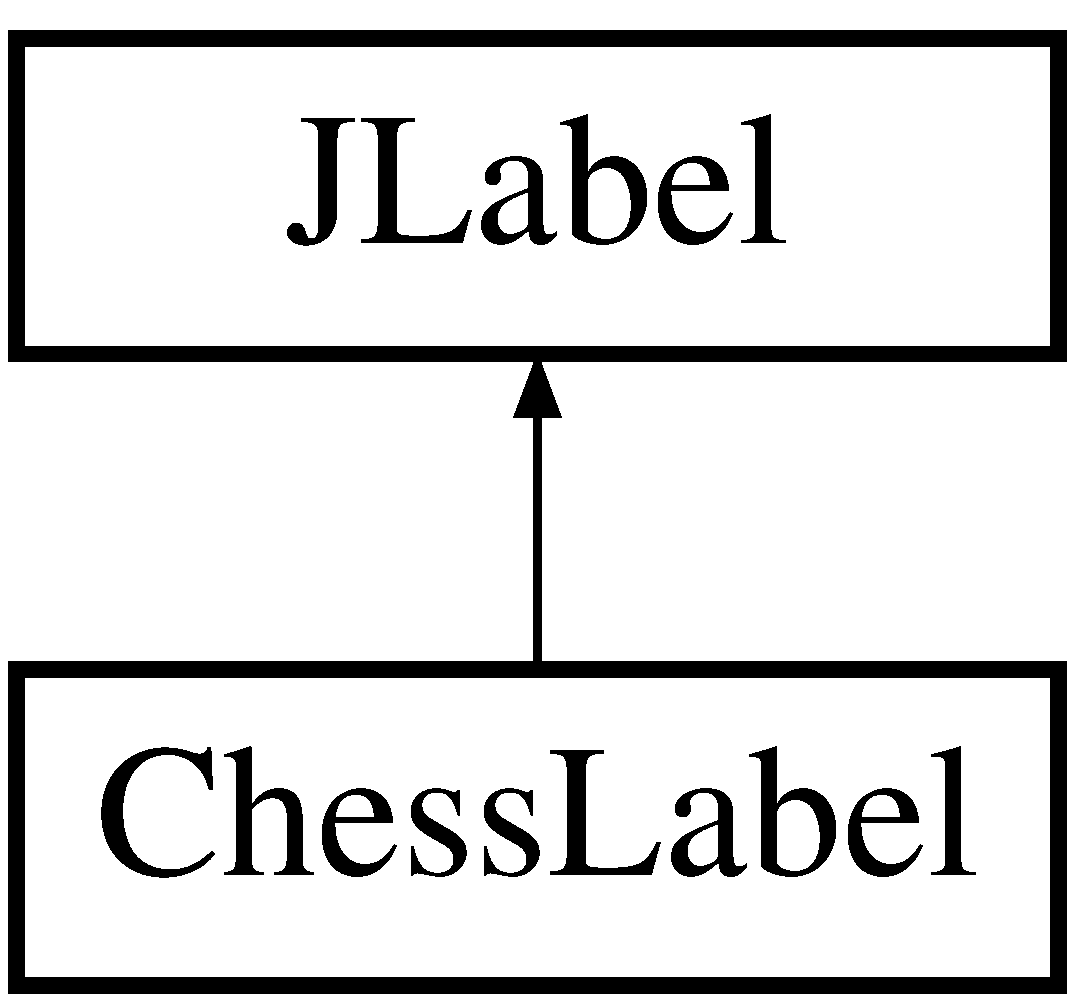
\includegraphics[height=2.000000cm]{class_chess_label}
\end{center}
\end{figure}


The documentation for this class was generated from the following file\+:\begin{DoxyCompactItemize}
\item 
src/Chess\+Label.\+java\end{DoxyCompactItemize}

\hypertarget{class_game}{}\section{Game Class Reference}
\label{class_game}\index{Game@{Game}}
\subsection*{Static Public Member Functions}
\begin{DoxyCompactItemize}
\item 
\hypertarget{class_game_ae52595a27ac1b327b05db2129ad81fca}{}static void {\bfseries main} (String\mbox{[}$\,$\mbox{]} args)\label{class_game_ae52595a27ac1b327b05db2129ad81fca}

\end{DoxyCompactItemize}


The documentation for this class was generated from the following file\+:\begin{DoxyCompactItemize}
\item 
src/Game.\+java\end{DoxyCompactItemize}

\hypertarget{class_hopper}{}\section{Hopper Class Reference}
\label{class_hopper}\index{Hopper@{Hopper}}
Inheritance diagram for Hopper\+:\begin{figure}[H]
\begin{center}
\leavevmode
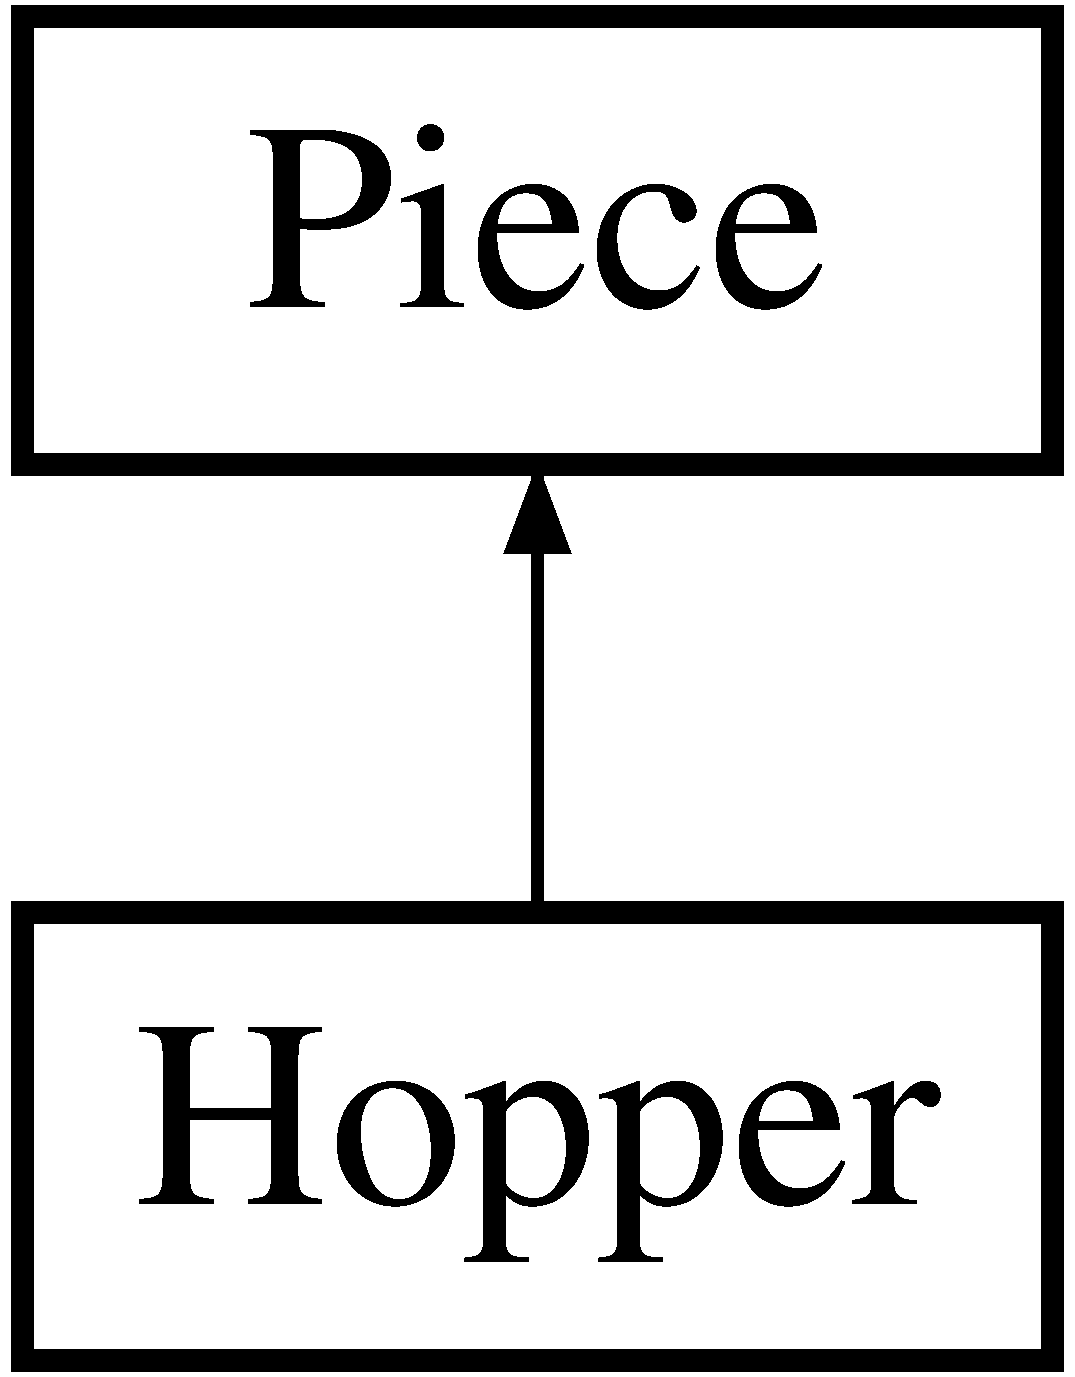
\includegraphics[height=2.000000cm]{class_hopper}
\end{center}
\end{figure}
\subsection*{Public Member Functions}
\begin{DoxyCompactItemize}
\item 
\hyperlink{class_hopper_a57319462bb507d517138e62c6a4fcbfb}{Hopper} (boolean color, int x\+Coord, int y\+Coord)
\item 
boolean \hyperlink{class_hopper_a4215ddac266467545aa9e4213567ca05}{is\+Valid\+Move} (\hyperlink{class_board}{Board} board, int to\+X, int to\+Y)
\end{DoxyCompactItemize}
\subsection*{Additional Inherited Members}


\subsection{Constructor \& Destructor Documentation}
\hypertarget{class_hopper_a57319462bb507d517138e62c6a4fcbfb}{}\index{Hopper@{Hopper}!Hopper@{Hopper}}
\index{Hopper@{Hopper}!Hopper@{Hopper}}
\subsubsection[{Hopper}]{\setlength{\rightskip}{0pt plus 5cm}Hopper.\+Hopper (
\begin{DoxyParamCaption}
\item[{boolean}]{color, }
\item[{int}]{x\+Coord, }
\item[{int}]{y\+Coord}
\end{DoxyParamCaption}
)}\label{class_hopper_a57319462bb507d517138e62c6a4fcbfb}
\hyperlink{class_hopper}{Hopper} is a knight that moves farther 
\begin{DoxyParams}{Parameters}
{\em color} & \\
\hline
{\em x\+Coord} & \\
\hline
{\em y\+Coord} & \\
\hline
\end{DoxyParams}


\subsection{Member Function Documentation}
\hypertarget{class_hopper_a4215ddac266467545aa9e4213567ca05}{}\index{Hopper@{Hopper}!is\+Valid\+Move@{is\+Valid\+Move}}
\index{is\+Valid\+Move@{is\+Valid\+Move}!Hopper@{Hopper}}
\subsubsection[{is\+Valid\+Move}]{\setlength{\rightskip}{0pt plus 5cm}boolean Hopper.\+is\+Valid\+Move (
\begin{DoxyParamCaption}
\item[{{\bf Board}}]{board, }
\item[{int}]{to\+X, }
\item[{int}]{to\+Y}
\end{DoxyParamCaption}
)}\label{class_hopper_a4215ddac266467545aa9e4213567ca05}
Check if Valid Move 
\begin{DoxyParams}{Parameters}
{\em board} & \\
\hline
{\em to\+X} & \\
\hline
{\em to\+Y} & \\
\hline
\end{DoxyParams}
\begin{DoxyReturn}{Returns}

\end{DoxyReturn}


The documentation for this class was generated from the following file\+:\begin{DoxyCompactItemize}
\item 
src/Hopper.\+java\end{DoxyCompactItemize}

\hypertarget{class_hopper_test}{}\section{Hopper\+Test Class Reference}
\label{class_hopper_test}\index{Hopper\+Test@{Hopper\+Test}}
\subsection*{Public Member Functions}
\begin{DoxyCompactItemize}
\item 
\hypertarget{class_hopper_test_accb0b9246afedc2cbaa1da02734a2456}{}void {\bfseries test\+Simple\+Move} ()  throws Exception \label{class_hopper_test_accb0b9246afedc2cbaa1da02734a2456}

\item 
\hypertarget{class_hopper_test_ac2df8ef8e7c775e01fc61ea396b9d32e}{}void {\bfseries test\+Capture} ()  throws Exception \label{class_hopper_test_ac2df8ef8e7c775e01fc61ea396b9d32e}

\item 
\hypertarget{class_hopper_test_a15310aece7aa8d72330606f185dba541}{}void {\bfseries test\+Illegal\+Move} ()  throws Exception \label{class_hopper_test_a15310aece7aa8d72330606f185dba541}

\end{DoxyCompactItemize}


The documentation for this class was generated from the following file\+:\begin{DoxyCompactItemize}
\item 
Test/Hopper\+Test.\+java\end{DoxyCompactItemize}

\hypertarget{class_juggernaut}{}\section{Juggernaut Class Reference}
\label{class_juggernaut}\index{Juggernaut@{Juggernaut}}
Inheritance diagram for Juggernaut\+:\begin{figure}[H]
\begin{center}
\leavevmode
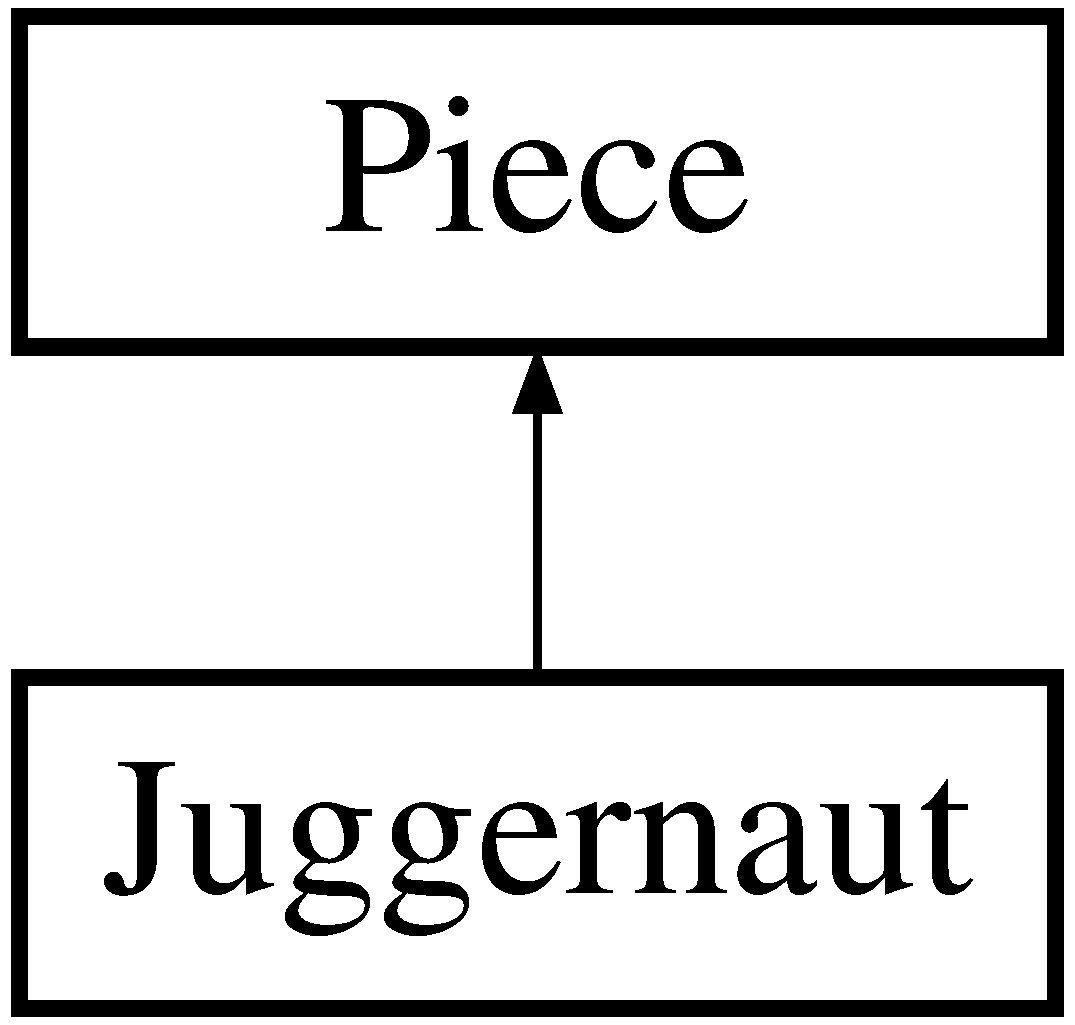
\includegraphics[height=2.000000cm]{class_juggernaut}
\end{center}
\end{figure}
\subsection*{Public Member Functions}
\begin{DoxyCompactItemize}
\item 
\hyperlink{class_juggernaut_ad574ceb708b62c6fb4b384f4f177bcdd}{Juggernaut} (boolean color, int x\+Coord, int y\+Coord)
\item 
boolean \hyperlink{class_juggernaut_a8b64c330d23e05e8e5721d28a01ad084}{is\+Valid\+Move} (\hyperlink{class_board}{Board} board, int to\+X, int to\+Y)
\end{DoxyCompactItemize}
\subsection*{Additional Inherited Members}


\subsection{Constructor \& Destructor Documentation}
\hypertarget{class_juggernaut_ad574ceb708b62c6fb4b384f4f177bcdd}{}\index{Juggernaut@{Juggernaut}!Juggernaut@{Juggernaut}}
\index{Juggernaut@{Juggernaut}!Juggernaut@{Juggernaut}}
\subsubsection[{Juggernaut}]{\setlength{\rightskip}{0pt plus 5cm}Juggernaut.\+Juggernaut (
\begin{DoxyParamCaption}
\item[{boolean}]{color, }
\item[{int}]{x\+Coord, }
\item[{int}]{y\+Coord}
\end{DoxyParamCaption}
)}\label{class_juggernaut_ad574ceb708b62c6fb4b384f4f177bcdd}
\hyperlink{class_juggernaut}{Juggernaut} \hyperlink{class_rook}{Rook} without collisions 
\begin{DoxyParams}{Parameters}
{\em color} & \\
\hline
{\em x\+Coord} & \\
\hline
{\em y\+Coord} & \\
\hline
\end{DoxyParams}


\subsection{Member Function Documentation}
\hypertarget{class_juggernaut_a8b64c330d23e05e8e5721d28a01ad084}{}\index{Juggernaut@{Juggernaut}!is\+Valid\+Move@{is\+Valid\+Move}}
\index{is\+Valid\+Move@{is\+Valid\+Move}!Juggernaut@{Juggernaut}}
\subsubsection[{is\+Valid\+Move}]{\setlength{\rightskip}{0pt plus 5cm}boolean Juggernaut.\+is\+Valid\+Move (
\begin{DoxyParamCaption}
\item[{{\bf Board}}]{board, }
\item[{int}]{to\+X, }
\item[{int}]{to\+Y}
\end{DoxyParamCaption}
)}\label{class_juggernaut_a8b64c330d23e05e8e5721d28a01ad084}
Check if Valid Move 
\begin{DoxyParams}{Parameters}
{\em board} & \\
\hline
{\em to\+X} & \\
\hline
{\em to\+Y} & \\
\hline
\end{DoxyParams}
\begin{DoxyReturn}{Returns}

\end{DoxyReturn}


The documentation for this class was generated from the following file\+:\begin{DoxyCompactItemize}
\item 
src/Juggernaut.\+java\end{DoxyCompactItemize}

\hypertarget{class_juggernaut_test}{}\section{Juggernaut\+Test Class Reference}
\label{class_juggernaut_test}\index{Juggernaut\+Test@{Juggernaut\+Test}}
\subsection*{Public Member Functions}
\begin{DoxyCompactItemize}
\item 
\hypertarget{class_juggernaut_test_a10642eab884fa12d22017b7c88886ae6}{}void {\bfseries test\+Simple\+Move} ()  throws Exception \label{class_juggernaut_test_a10642eab884fa12d22017b7c88886ae6}

\item 
\hypertarget{class_juggernaut_test_a7b2d4cc81b3fa2116d23a961cae50f1b}{}void {\bfseries test\+Capture} ()  throws Exception \label{class_juggernaut_test_a7b2d4cc81b3fa2116d23a961cae50f1b}

\item 
\hypertarget{class_juggernaut_test_aed8ab48bc46a7d8679ede8cd876ff36e}{}void {\bfseries test\+Capture\+Through\+Piece} ()  throws Exception \label{class_juggernaut_test_aed8ab48bc46a7d8679ede8cd876ff36e}

\item 
\hypertarget{class_juggernaut_test_aa39748f749c7cf3f7876c4a7e236c604}{}void {\bfseries test\+Illegal\+Move} ()  throws Exception \label{class_juggernaut_test_aa39748f749c7cf3f7876c4a7e236c604}

\end{DoxyCompactItemize}


The documentation for this class was generated from the following file\+:\begin{DoxyCompactItemize}
\item 
Test/Juggernaut\+Test.\+java\end{DoxyCompactItemize}

\hypertarget{class_king}{}\section{King Class Reference}
\label{class_king}\index{King@{King}}
Inheritance diagram for King\+:\begin{figure}[H]
\begin{center}
\leavevmode
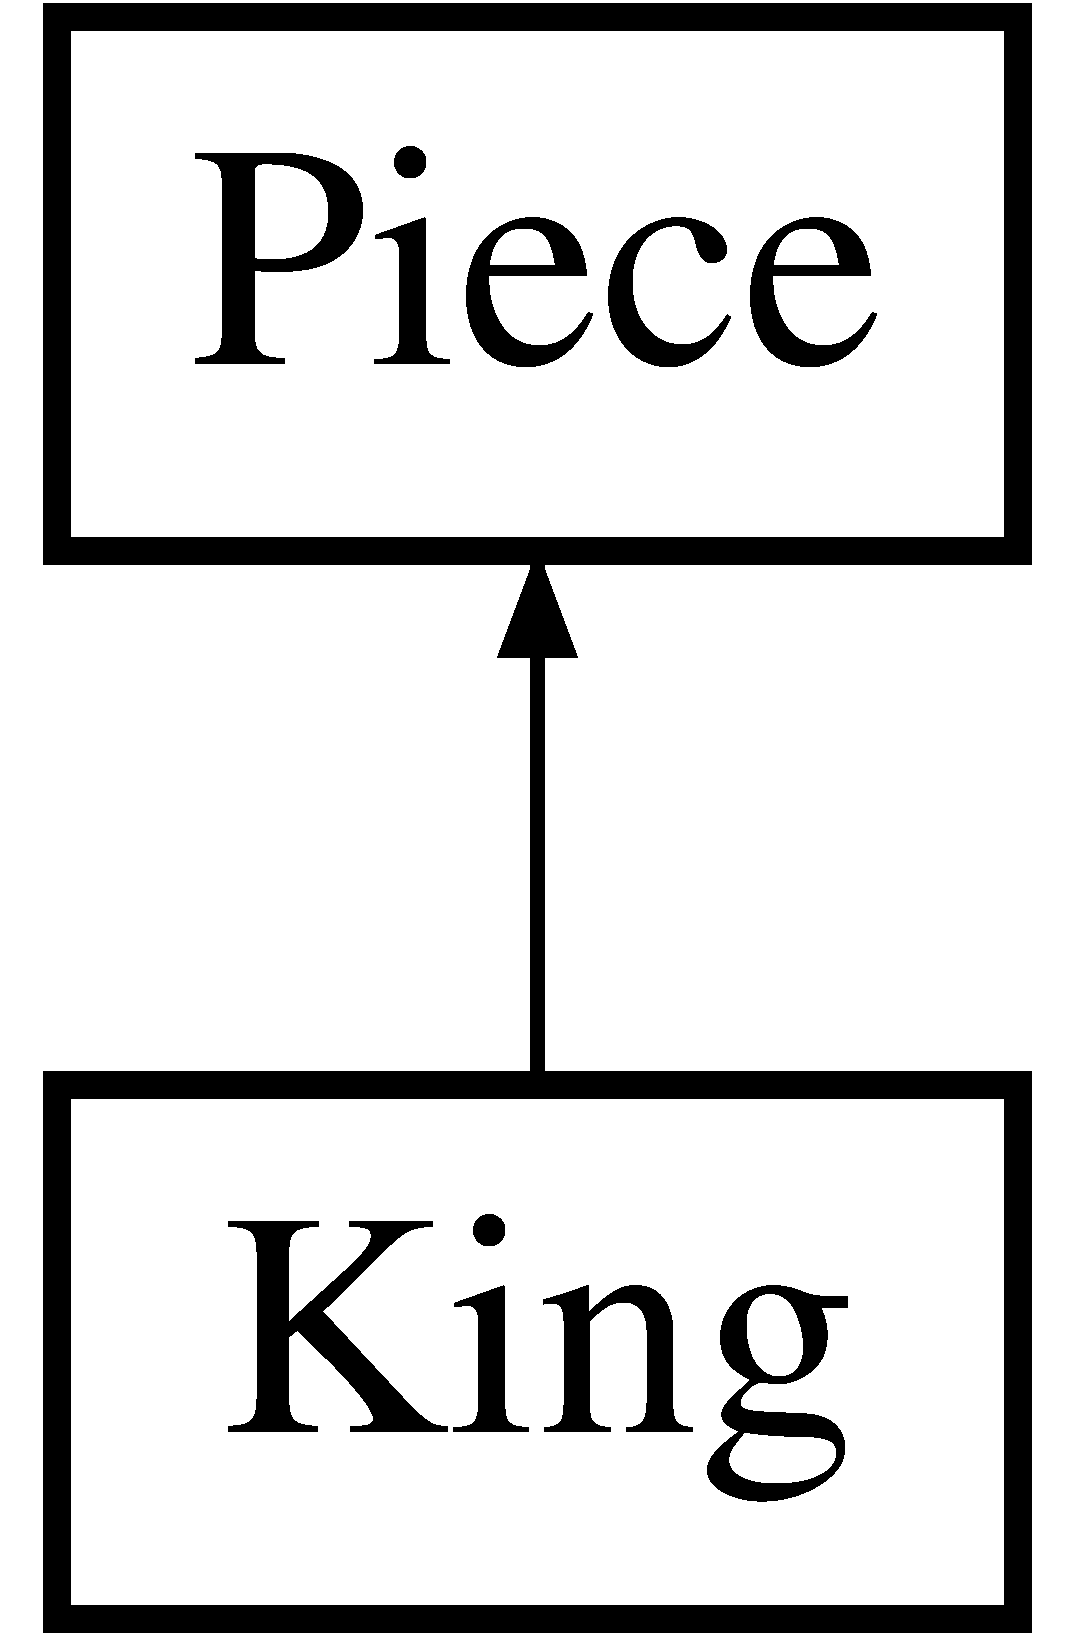
\includegraphics[height=2.000000cm]{class_king}
\end{center}
\end{figure}
\subsection*{Public Member Functions}
\begin{DoxyCompactItemize}
\item 
\hyperlink{class_king_ad96c3a3a36b0aa70c379979ebf3641cf}{King} (boolean color, int x\+Coord, int y\+Coord)
\item 
boolean \hyperlink{class_king_a9c55d90f6fe845140c90396f9624cd17}{is\+Valid\+Move} (\hyperlink{class_board}{Board} board, int to\+X, int to\+Y)
\end{DoxyCompactItemize}
\subsection*{Additional Inherited Members}


\subsection{Constructor \& Destructor Documentation}
\hypertarget{class_king_ad96c3a3a36b0aa70c379979ebf3641cf}{}\index{King@{King}!King@{King}}
\index{King@{King}!King@{King}}
\subsubsection[{King}]{\setlength{\rightskip}{0pt plus 5cm}King.\+King (
\begin{DoxyParamCaption}
\item[{boolean}]{color, }
\item[{int}]{x\+Coord, }
\item[{int}]{y\+Coord}
\end{DoxyParamCaption}
)}\label{class_king_ad96c3a3a36b0aa70c379979ebf3641cf}
\hyperlink{class_king}{King} Constructor 
\begin{DoxyParams}{Parameters}
{\em color} & \\
\hline
{\em x\+Coord} & \\
\hline
{\em y\+Coord} & \\
\hline
\end{DoxyParams}


\subsection{Member Function Documentation}
\hypertarget{class_king_a9c55d90f6fe845140c90396f9624cd17}{}\index{King@{King}!is\+Valid\+Move@{is\+Valid\+Move}}
\index{is\+Valid\+Move@{is\+Valid\+Move}!King@{King}}
\subsubsection[{is\+Valid\+Move}]{\setlength{\rightskip}{0pt plus 5cm}boolean King.\+is\+Valid\+Move (
\begin{DoxyParamCaption}
\item[{{\bf Board}}]{board, }
\item[{int}]{to\+X, }
\item[{int}]{to\+Y}
\end{DoxyParamCaption}
)}\label{class_king_a9c55d90f6fe845140c90396f9624cd17}
Check if Valid Move for \hyperlink{class_king}{King} 
\begin{DoxyParams}{Parameters}
{\em board} & \\
\hline
{\em to\+X} & \\
\hline
{\em to\+Y} & \\
\hline
\end{DoxyParams}
\begin{DoxyReturn}{Returns}

\end{DoxyReturn}


The documentation for this class was generated from the following file\+:\begin{DoxyCompactItemize}
\item 
src/King.\+java\end{DoxyCompactItemize}

\hypertarget{class_king_test}{}\section{King\+Test Class Reference}
\label{class_king_test}\index{King\+Test@{King\+Test}}
\subsection*{Public Member Functions}
\begin{DoxyCompactItemize}
\item 
\hypertarget{class_king_test_a027b1ece1e12a4bbc44b7ecc3bf19a45}{}void {\bfseries test\+Simple\+Move} ()  throws Exception \label{class_king_test_a027b1ece1e12a4bbc44b7ecc3bf19a45}

\item 
\hypertarget{class_king_test_af93043b862ff76688ca8977aea5c8448}{}void {\bfseries test\+Capture} ()  throws Exception \label{class_king_test_af93043b862ff76688ca8977aea5c8448}

\item 
\hypertarget{class_king_test_adfdf4d1888d505c1281ce1020bf5154f}{}void {\bfseries test\+Illegal\+Move} ()  throws Exception \label{class_king_test_adfdf4d1888d505c1281ce1020bf5154f}

\end{DoxyCompactItemize}


The documentation for this class was generated from the following file\+:\begin{DoxyCompactItemize}
\item 
Test/King\+Test.\+java\end{DoxyCompactItemize}

\hypertarget{class_knight}{}\section{Knight Class Reference}
\label{class_knight}\index{Knight@{Knight}}
Inheritance diagram for Knight\+:\begin{figure}[H]
\begin{center}
\leavevmode
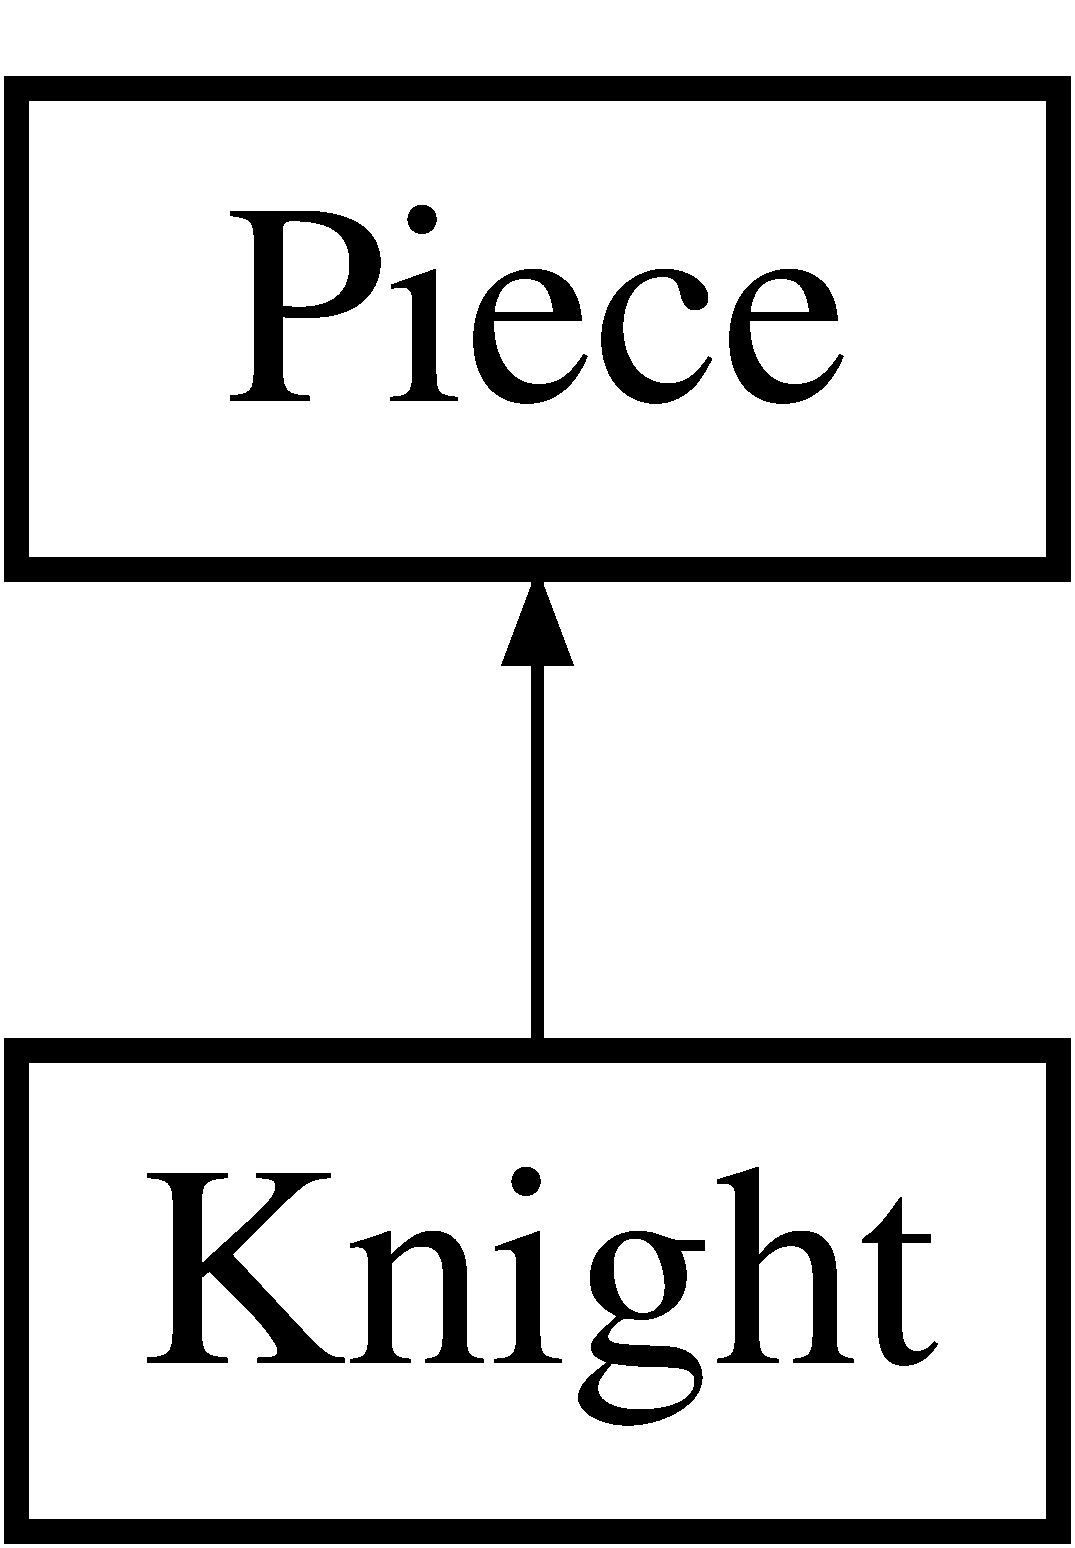
\includegraphics[height=2.000000cm]{class_knight}
\end{center}
\end{figure}
\subsection*{Public Member Functions}
\begin{DoxyCompactItemize}
\item 
\hyperlink{class_knight_a9169d42dbaa01077c597ca52a908a954}{Knight} (boolean color, int x\+Coord, int y\+Coord)
\item 
boolean \hyperlink{class_knight_a078def1f1a859f749f21abbf33dc51e3}{is\+Valid\+Move} (\hyperlink{class_board}{Board} board, int to\+X, int to\+Y)
\end{DoxyCompactItemize}
\subsection*{Additional Inherited Members}


\subsection{Constructor \& Destructor Documentation}
\hypertarget{class_knight_a9169d42dbaa01077c597ca52a908a954}{}\index{Knight@{Knight}!Knight@{Knight}}
\index{Knight@{Knight}!Knight@{Knight}}
\subsubsection[{Knight}]{\setlength{\rightskip}{0pt plus 5cm}Knight.\+Knight (
\begin{DoxyParamCaption}
\item[{boolean}]{color, }
\item[{int}]{x\+Coord, }
\item[{int}]{y\+Coord}
\end{DoxyParamCaption}
)}\label{class_knight_a9169d42dbaa01077c597ca52a908a954}
\hyperlink{class_knight}{Knight} Constructor 
\begin{DoxyParams}{Parameters}
{\em color} & \\
\hline
{\em x\+Coord} & \\
\hline
{\em y\+Coord} & \\
\hline
\end{DoxyParams}


\subsection{Member Function Documentation}
\hypertarget{class_knight_a078def1f1a859f749f21abbf33dc51e3}{}\index{Knight@{Knight}!is\+Valid\+Move@{is\+Valid\+Move}}
\index{is\+Valid\+Move@{is\+Valid\+Move}!Knight@{Knight}}
\subsubsection[{is\+Valid\+Move}]{\setlength{\rightskip}{0pt plus 5cm}boolean Knight.\+is\+Valid\+Move (
\begin{DoxyParamCaption}
\item[{{\bf Board}}]{board, }
\item[{int}]{to\+X, }
\item[{int}]{to\+Y}
\end{DoxyParamCaption}
)}\label{class_knight_a078def1f1a859f749f21abbf33dc51e3}
Check if valid move for \hyperlink{class_knight}{Knight} 
\begin{DoxyParams}{Parameters}
{\em board} & \\
\hline
{\em to\+X} & \\
\hline
{\em to\+Y} & \\
\hline
\end{DoxyParams}
\begin{DoxyReturn}{Returns}

\end{DoxyReturn}


The documentation for this class was generated from the following file\+:\begin{DoxyCompactItemize}
\item 
src/Knight.\+java\end{DoxyCompactItemize}

\hypertarget{class_knight_test}{}\section{Knight\+Test Class Reference}
\label{class_knight_test}\index{Knight\+Test@{Knight\+Test}}
\subsection*{Public Member Functions}
\begin{DoxyCompactItemize}
\item 
\hypertarget{class_knight_test_a73de9571a449a308819f74a48aca89d1}{}void {\bfseries test\+Simple\+Move} ()  throws Exception \label{class_knight_test_a73de9571a449a308819f74a48aca89d1}

\item 
\hypertarget{class_knight_test_ac1854121a956826ca37e70ff966e5ccf}{}void {\bfseries test\+Capture} ()  throws Exception\label{class_knight_test_ac1854121a956826ca37e70ff966e5ccf}

\item 
\hypertarget{class_knight_test_ac8113b7b91cf88b68f610cc5c8348666}{}void {\bfseries test\+Illegal\+Move} ()  throws Exception \label{class_knight_test_ac8113b7b91cf88b68f610cc5c8348666}

\end{DoxyCompactItemize}


The documentation for this class was generated from the following file\+:\begin{DoxyCompactItemize}
\item 
Test/Knight\+Test.\+java\end{DoxyCompactItemize}

\hypertarget{class_pawn}{}\section{Pawn Class Reference}
\label{class_pawn}\index{Pawn@{Pawn}}
Inheritance diagram for Pawn\+:\begin{figure}[H]
\begin{center}
\leavevmode
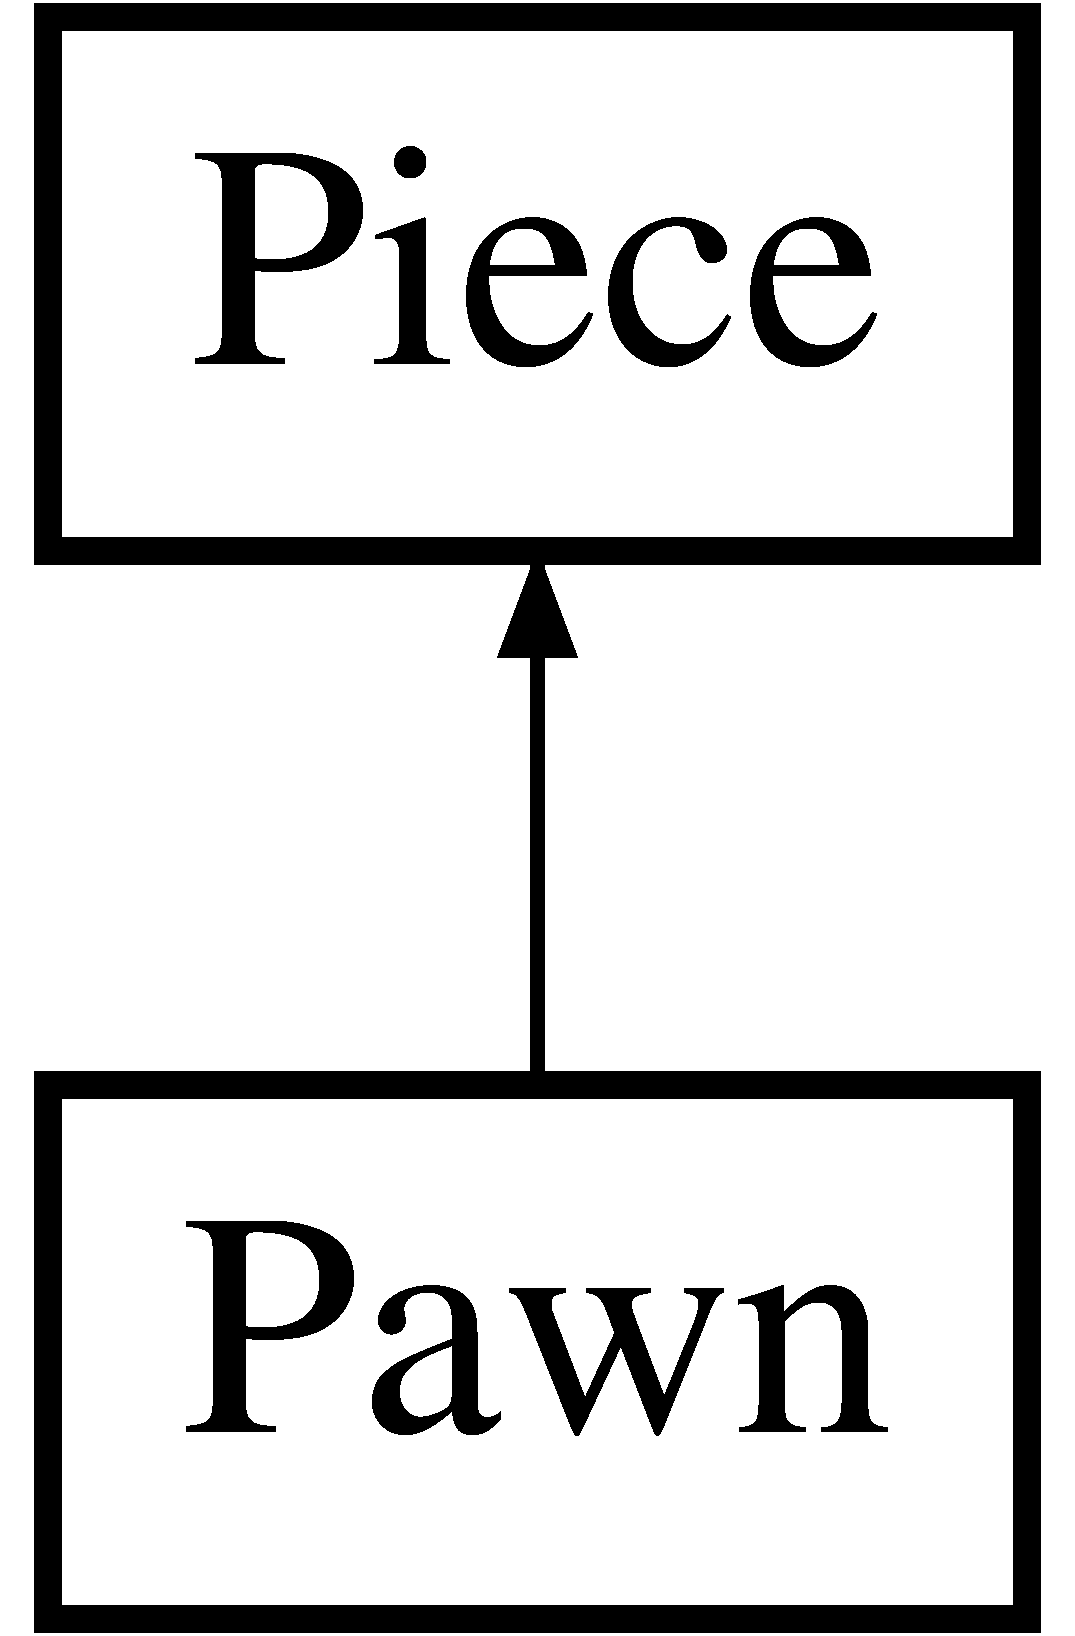
\includegraphics[height=2.000000cm]{class_pawn}
\end{center}
\end{figure}
\subsection*{Public Member Functions}
\begin{DoxyCompactItemize}
\item 
\hyperlink{class_pawn_ae1cc2820b499ba3ec756492b9841483b}{Pawn} (boolean color, int x\+Coord, int y\+Coord)
\item 
boolean \hyperlink{class_pawn_a71015ece742ecd8b50265f83fdd26d3d}{is\+Valid\+Move} (\hyperlink{class_board}{Board} board, int to\+X, int to\+Y)
\end{DoxyCompactItemize}
\subsection*{Additional Inherited Members}


\subsection{Constructor \& Destructor Documentation}
\hypertarget{class_pawn_ae1cc2820b499ba3ec756492b9841483b}{}\index{Pawn@{Pawn}!Pawn@{Pawn}}
\index{Pawn@{Pawn}!Pawn@{Pawn}}
\subsubsection[{Pawn}]{\setlength{\rightskip}{0pt plus 5cm}Pawn.\+Pawn (
\begin{DoxyParamCaption}
\item[{boolean}]{color, }
\item[{int}]{x\+Coord, }
\item[{int}]{y\+Coord}
\end{DoxyParamCaption}
)}\label{class_pawn_ae1cc2820b499ba3ec756492b9841483b}
\hyperlink{class_pawn}{Pawn} Constructor 
\begin{DoxyParams}{Parameters}
{\em color} & \\
\hline
{\em x\+Coord} & \\
\hline
{\em y\+Coord} & \\
\hline
\end{DoxyParams}


\subsection{Member Function Documentation}
\hypertarget{class_pawn_a71015ece742ecd8b50265f83fdd26d3d}{}\index{Pawn@{Pawn}!is\+Valid\+Move@{is\+Valid\+Move}}
\index{is\+Valid\+Move@{is\+Valid\+Move}!Pawn@{Pawn}}
\subsubsection[{is\+Valid\+Move}]{\setlength{\rightskip}{0pt plus 5cm}boolean Pawn.\+is\+Valid\+Move (
\begin{DoxyParamCaption}
\item[{{\bf Board}}]{board, }
\item[{int}]{to\+X, }
\item[{int}]{to\+Y}
\end{DoxyParamCaption}
)}\label{class_pawn_a71015ece742ecd8b50265f83fdd26d3d}
Check if Move is Valid for \hyperlink{class_pawn}{Pawn} 
\begin{DoxyParams}{Parameters}
{\em board} & \\
\hline
{\em to\+X} & \\
\hline
{\em to\+Y} & \\
\hline
\end{DoxyParams}
\begin{DoxyReturn}{Returns}

\end{DoxyReturn}


The documentation for this class was generated from the following file\+:\begin{DoxyCompactItemize}
\item 
src/Pawn.\+java\end{DoxyCompactItemize}

\hypertarget{class_pawn_test}{}\section{Pawn\+Test Class Reference}
\label{class_pawn_test}\index{Pawn\+Test@{Pawn\+Test}}
\subsection*{Public Member Functions}
\begin{DoxyCompactItemize}
\item 
\hypertarget{class_pawn_test_a5fc5a41879f2e241700113fdf6f40395}{}void {\bfseries test\+Simple\+Move} ()  throws Exception \label{class_pawn_test_a5fc5a41879f2e241700113fdf6f40395}

\item 
\hypertarget{class_pawn_test_a844d85f5e8d5292b920a8367d94831b2}{}void {\bfseries test\+Capture} ()  throws Exception \label{class_pawn_test_a844d85f5e8d5292b920a8367d94831b2}

\item 
\hypertarget{class_pawn_test_aa70e6edb95a5d9f6776809fd1ba4abaf}{}void {\bfseries test\+First\+Move} ()  throws Exception \label{class_pawn_test_aa70e6edb95a5d9f6776809fd1ba4abaf}

\end{DoxyCompactItemize}


The documentation for this class was generated from the following file\+:\begin{DoxyCompactItemize}
\item 
Test/Pawn\+Test.\+java\end{DoxyCompactItemize}

\hypertarget{class_piece}{}\section{Piece Class Reference}
\label{class_piece}\index{Piece@{Piece}}
Inheritance diagram for Piece\+:\begin{figure}[H]
\begin{center}
\leavevmode
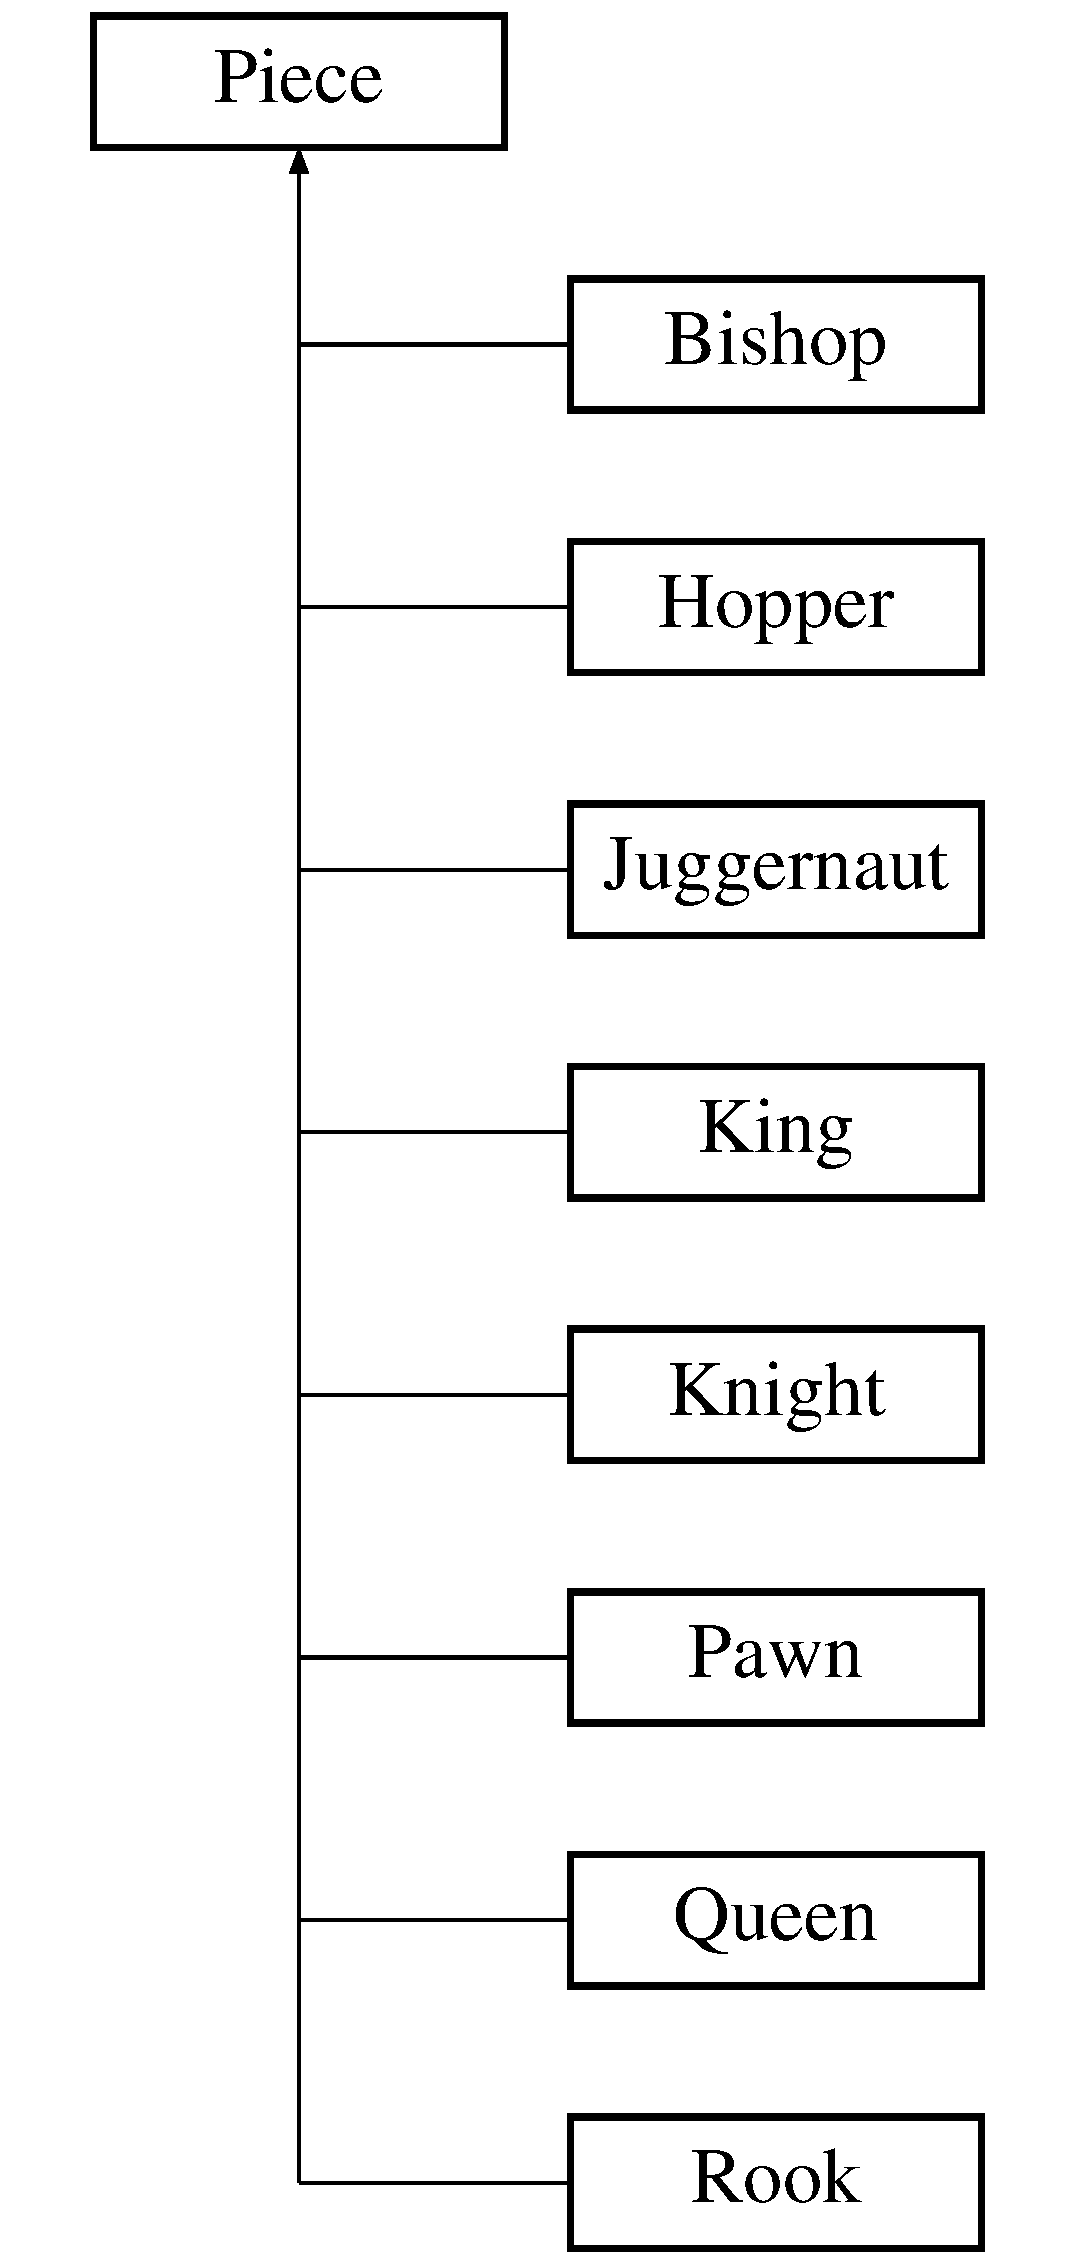
\includegraphics[height=9.000000cm]{class_piece}
\end{center}
\end{figure}
\subsection*{Public Member Functions}
\begin{DoxyCompactItemize}
\item 
\hyperlink{class_piece_a3a01b38c9778e479443e782a9ad1b97d}{Piece} (boolean color, int x\+Coord, int y\+Coord)
\item 
boolean \hyperlink{class_piece_a423f42b9f07bd5edf2faba8753083e2f}{piece\+In\+Way} (\hyperlink{class_board}{Board} board, int to\+X, int to\+Y)
\item 
boolean \hyperlink{class_piece_a2b843e1dee9e155eb8e99e3411fd27e6}{get\+Color} ()
\item 
void \hyperlink{class_piece_acf1f3826e59942648be325f3c8f48800}{exec\+Move} (\hyperlink{class_board}{Board} board, \hyperlink{class_player}{Player} player, \hyperlink{class_piece}{Piece} piece, int to\+X, int to\+Y)
\item 
boolean \hyperlink{class_piece_a246d5e14b444acc54178b3c0ca353a06}{is\+On\+Board} (\hyperlink{class_board}{Board} board, int to\+X, int to\+Y)
\end{DoxyCompactItemize}
\subsection*{Public Attributes}
\begin{DoxyCompactItemize}
\item 
\hypertarget{class_piece_a05d7aa69f6299e0f2ca0268dbd1cf1de}{}int {\bfseries x\+Coord}\label{class_piece_a05d7aa69f6299e0f2ca0268dbd1cf1de}

\item 
\hypertarget{class_piece_a2d5620bb565c94487f3f8ee3b556aee1}{}int {\bfseries y\+Coord}\label{class_piece_a2d5620bb565c94487f3f8ee3b556aee1}

\item 
\hypertarget{class_piece_acc17b96cb4e5e55946afedc9435b2936}{}boolean {\bfseries color}\label{class_piece_acc17b96cb4e5e55946afedc9435b2936}

\end{DoxyCompactItemize}


\subsection{Constructor \& Destructor Documentation}
\hypertarget{class_piece_a3a01b38c9778e479443e782a9ad1b97d}{}\index{Piece@{Piece}!Piece@{Piece}}
\index{Piece@{Piece}!Piece@{Piece}}
\subsubsection[{Piece}]{\setlength{\rightskip}{0pt plus 5cm}Piece.\+Piece (
\begin{DoxyParamCaption}
\item[{boolean}]{color, }
\item[{int}]{x\+Coord, }
\item[{int}]{y\+Coord}
\end{DoxyParamCaption}
)}\label{class_piece_a3a01b38c9778e479443e782a9ad1b97d}
\hyperlink{class_piece}{Piece} Constructor 
\begin{DoxyParams}{Parameters}
{\em color} & \\
\hline
{\em x\+Coord} & \\
\hline
{\em y\+Coord} & \\
\hline
\end{DoxyParams}


\subsection{Member Function Documentation}
\hypertarget{class_piece_acf1f3826e59942648be325f3c8f48800}{}\index{Piece@{Piece}!exec\+Move@{exec\+Move}}
\index{exec\+Move@{exec\+Move}!Piece@{Piece}}
\subsubsection[{exec\+Move}]{\setlength{\rightskip}{0pt plus 5cm}void Piece.\+exec\+Move (
\begin{DoxyParamCaption}
\item[{{\bf Board}}]{board, }
\item[{{\bf Player}}]{player, }
\item[{{\bf Piece}}]{piece, }
\item[{int}]{to\+X, }
\item[{int}]{to\+Y}
\end{DoxyParamCaption}
)}\label{class_piece_acf1f3826e59942648be325f3c8f48800}
Execute Move/\+Capture \hyperlink{class_piece}{Piece} 
\begin{DoxyParams}{Parameters}
{\em board} & \\
\hline
{\em player} & \\
\hline
{\em to\+X} & \\
\hline
{\em to\+Y} & \\
\hline
\end{DoxyParams}
\hypertarget{class_piece_a2b843e1dee9e155eb8e99e3411fd27e6}{}\index{Piece@{Piece}!get\+Color@{get\+Color}}
\index{get\+Color@{get\+Color}!Piece@{Piece}}
\subsubsection[{get\+Color}]{\setlength{\rightskip}{0pt plus 5cm}boolean Piece.\+get\+Color (
\begin{DoxyParamCaption}
{}
\end{DoxyParamCaption}
)}\label{class_piece_a2b843e1dee9e155eb8e99e3411fd27e6}
Retrieve color of \hyperlink{class_piece}{Piece} \begin{DoxyReturn}{Returns}

\end{DoxyReturn}
\hypertarget{class_piece_a246d5e14b444acc54178b3c0ca353a06}{}\index{Piece@{Piece}!is\+On\+Board@{is\+On\+Board}}
\index{is\+On\+Board@{is\+On\+Board}!Piece@{Piece}}
\subsubsection[{is\+On\+Board}]{\setlength{\rightskip}{0pt plus 5cm}boolean Piece.\+is\+On\+Board (
\begin{DoxyParamCaption}
\item[{{\bf Board}}]{board, }
\item[{int}]{to\+X, }
\item[{int}]{to\+Y}
\end{DoxyParamCaption}
)}\label{class_piece_a246d5e14b444acc54178b3c0ca353a06}
Verify that piece is on board 
\begin{DoxyParams}{Parameters}
{\em board} & \\
\hline
{\em to\+X} & \\
\hline
{\em to\+Y} & \\
\hline
\end{DoxyParams}
\begin{DoxyReturn}{Returns}

\end{DoxyReturn}
\hypertarget{class_piece_a423f42b9f07bd5edf2faba8753083e2f}{}\index{Piece@{Piece}!piece\+In\+Way@{piece\+In\+Way}}
\index{piece\+In\+Way@{piece\+In\+Way}!Piece@{Piece}}
\subsubsection[{piece\+In\+Way}]{\setlength{\rightskip}{0pt plus 5cm}boolean Piece.\+piece\+In\+Way (
\begin{DoxyParamCaption}
\item[{{\bf Board}}]{board, }
\item[{int}]{to\+X, }
\item[{int}]{to\+Y}
\end{DoxyParamCaption}
)}\label{class_piece_a423f42b9f07bd5edf2faba8753083e2f}
Check if piece obstructs movement 
\begin{DoxyParams}{Parameters}
{\em board} & \\
\hline
{\em to\+X} & \\
\hline
{\em to\+Y} & \\
\hline
\end{DoxyParams}
\begin{DoxyReturn}{Returns}

\end{DoxyReturn}


The documentation for this class was generated from the following file\+:\begin{DoxyCompactItemize}
\item 
src/Piece.\+java\end{DoxyCompactItemize}

\hypertarget{class_player}{}\section{Player Class Reference}
\label{class_player}\index{Player@{Player}}
\subsection*{Public Member Functions}
\begin{DoxyCompactItemize}
\item 
\hyperlink{class_player_ae44e103cbf5ac9da4a6c7298cb7e431a}{Player} (boolean color)
\end{DoxyCompactItemize}
\subsection*{Static Public Member Functions}
\begin{DoxyCompactItemize}
\item 
static boolean \hyperlink{class_player_a5119de45fe4baf24f6781daa64a33f28}{get\+Color} ()
\end{DoxyCompactItemize}
\subsection*{Static Public Attributes}
\begin{DoxyCompactItemize}
\item 
\hypertarget{class_player_a3e7a6271c305b920b4dda6c98156d0ef}{}static final boolean {\bfseries white} = true\label{class_player_a3e7a6271c305b920b4dda6c98156d0ef}

\item 
\hypertarget{class_player_a719ad9a1a67db53c7b520a11676f405a}{}static final boolean {\bfseries black} = false\label{class_player_a719ad9a1a67db53c7b520a11676f405a}

\end{DoxyCompactItemize}


\subsection{Constructor \& Destructor Documentation}
\hypertarget{class_player_ae44e103cbf5ac9da4a6c7298cb7e431a}{}\index{Player@{Player}!Player@{Player}}
\index{Player@{Player}!Player@{Player}}
\subsubsection[{Player}]{\setlength{\rightskip}{0pt plus 5cm}Player.\+Player (
\begin{DoxyParamCaption}
\item[{boolean}]{color}
\end{DoxyParamCaption}
)}\label{class_player_ae44e103cbf5ac9da4a6c7298cb7e431a}
Constructor \hyperlink{class_player}{Player} 
\begin{DoxyParams}{Parameters}
{\em color} & \\
\hline
\end{DoxyParams}


\subsection{Member Function Documentation}
\hypertarget{class_player_a5119de45fe4baf24f6781daa64a33f28}{}\index{Player@{Player}!get\+Color@{get\+Color}}
\index{get\+Color@{get\+Color}!Player@{Player}}
\subsubsection[{get\+Color}]{\setlength{\rightskip}{0pt plus 5cm}static boolean Player.\+get\+Color (
\begin{DoxyParamCaption}
{}
\end{DoxyParamCaption}
)\hspace{0.3cm}{\ttfamily [static]}}\label{class_player_a5119de45fe4baf24f6781daa64a33f28}
Get Color \begin{DoxyReturn}{Returns}

\end{DoxyReturn}


The documentation for this class was generated from the following file\+:\begin{DoxyCompactItemize}
\item 
src/Player.\+java\end{DoxyCompactItemize}

\hypertarget{class_queen}{}\section{Queen Class Reference}
\label{class_queen}\index{Queen@{Queen}}
Inheritance diagram for Queen\+:\begin{figure}[H]
\begin{center}
\leavevmode
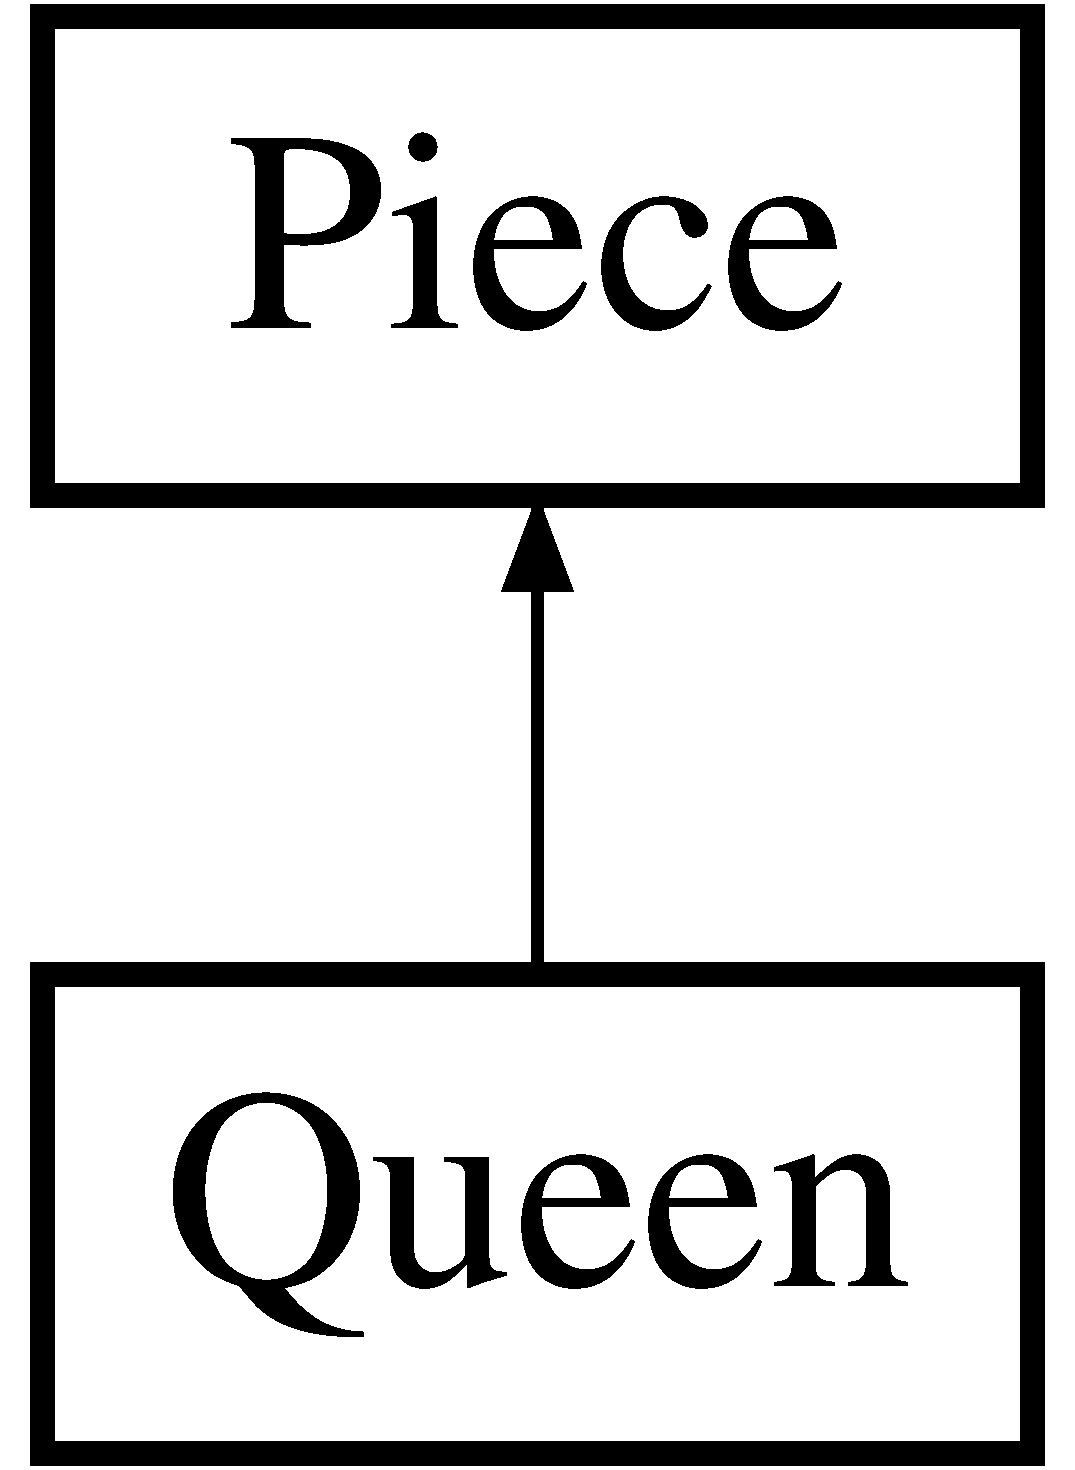
\includegraphics[height=2.000000cm]{class_queen}
\end{center}
\end{figure}
\subsection*{Public Member Functions}
\begin{DoxyCompactItemize}
\item 
\hyperlink{class_queen_a85b8dcbd96f1e792208f388fd7b55949}{Queen} (boolean color, int x\+Coord, int y\+Coord)
\item 
boolean \hyperlink{class_queen_a7f397d5f8f12549b3125d7b536d6eabb}{is\+Valid\+Move} (\hyperlink{class_board}{Board} board, int to\+X, int to\+Y)
\item 
boolean \hyperlink{class_queen_a6757f1972c7f9b6150e25bd0756d28db}{piece\+In\+Way\+Straight} (\hyperlink{class_board}{Board} board, int to\+X, int to\+Y)
\item 
boolean \hyperlink{class_queen_aa2e958bbb73dbe2ebd82e917d7a74e00}{piece\+In\+Way\+Diagonal} (\hyperlink{class_board}{Board} board, int to\+X, int to\+Y)
\end{DoxyCompactItemize}
\subsection*{Additional Inherited Members}


\subsection{Constructor \& Destructor Documentation}
\hypertarget{class_queen_a85b8dcbd96f1e792208f388fd7b55949}{}\index{Queen@{Queen}!Queen@{Queen}}
\index{Queen@{Queen}!Queen@{Queen}}
\subsubsection[{Queen}]{\setlength{\rightskip}{0pt plus 5cm}Queen.\+Queen (
\begin{DoxyParamCaption}
\item[{boolean}]{color, }
\item[{int}]{x\+Coord, }
\item[{int}]{y\+Coord}
\end{DoxyParamCaption}
)}\label{class_queen_a85b8dcbd96f1e792208f388fd7b55949}
\hyperlink{class_queen}{Queen} Constructor 
\begin{DoxyParams}{Parameters}
{\em color} & \\
\hline
{\em x\+Coord} & \\
\hline
{\em y\+Coord} & \\
\hline
\end{DoxyParams}


\subsection{Member Function Documentation}
\hypertarget{class_queen_a7f397d5f8f12549b3125d7b536d6eabb}{}\index{Queen@{Queen}!is\+Valid\+Move@{is\+Valid\+Move}}
\index{is\+Valid\+Move@{is\+Valid\+Move}!Queen@{Queen}}
\subsubsection[{is\+Valid\+Move}]{\setlength{\rightskip}{0pt plus 5cm}boolean Queen.\+is\+Valid\+Move (
\begin{DoxyParamCaption}
\item[{{\bf Board}}]{board, }
\item[{int}]{to\+X, }
\item[{int}]{to\+Y}
\end{DoxyParamCaption}
)}\label{class_queen_a7f397d5f8f12549b3125d7b536d6eabb}
Validate \hyperlink{class_queen}{Queen} move 
\begin{DoxyParams}{Parameters}
{\em board} & \\
\hline
{\em to\+X} & \\
\hline
{\em to\+Y} & \\
\hline
\end{DoxyParams}
\begin{DoxyReturn}{Returns}

\end{DoxyReturn}
\hypertarget{class_queen_aa2e958bbb73dbe2ebd82e917d7a74e00}{}\index{Queen@{Queen}!piece\+In\+Way\+Diagonal@{piece\+In\+Way\+Diagonal}}
\index{piece\+In\+Way\+Diagonal@{piece\+In\+Way\+Diagonal}!Queen@{Queen}}
\subsubsection[{piece\+In\+Way\+Diagonal}]{\setlength{\rightskip}{0pt plus 5cm}boolean Queen.\+piece\+In\+Way\+Diagonal (
\begin{DoxyParamCaption}
\item[{{\bf Board}}]{board, }
\item[{int}]{to\+X, }
\item[{int}]{to\+Y}
\end{DoxyParamCaption}
)}\label{class_queen_aa2e958bbb73dbe2ebd82e917d7a74e00}
Reuse \hyperlink{class_bishop}{Bishop} rules for collisions 
\begin{DoxyParams}{Parameters}
{\em board} & \\
\hline
{\em to\+X} & \\
\hline
{\em to\+Y} & \\
\hline
\end{DoxyParams}
\begin{DoxyReturn}{Returns}

\end{DoxyReturn}
\hypertarget{class_queen_a6757f1972c7f9b6150e25bd0756d28db}{}\index{Queen@{Queen}!piece\+In\+Way\+Straight@{piece\+In\+Way\+Straight}}
\index{piece\+In\+Way\+Straight@{piece\+In\+Way\+Straight}!Queen@{Queen}}
\subsubsection[{piece\+In\+Way\+Straight}]{\setlength{\rightskip}{0pt plus 5cm}boolean Queen.\+piece\+In\+Way\+Straight (
\begin{DoxyParamCaption}
\item[{{\bf Board}}]{board, }
\item[{int}]{to\+X, }
\item[{int}]{to\+Y}
\end{DoxyParamCaption}
)}\label{class_queen_a6757f1972c7f9b6150e25bd0756d28db}
Use \hyperlink{class_rook}{Rook} Rules for collisions 
\begin{DoxyParams}{Parameters}
{\em board} & \\
\hline
{\em to\+X} & \\
\hline
{\em to\+Y} & \\
\hline
\end{DoxyParams}
\begin{DoxyReturn}{Returns}

\end{DoxyReturn}


The documentation for this class was generated from the following file\+:\begin{DoxyCompactItemize}
\item 
src/Queen.\+java\end{DoxyCompactItemize}

\hypertarget{class_queen_test}{}\section{Queen\+Test Class Reference}
\label{class_queen_test}\index{Queen\+Test@{Queen\+Test}}
\subsection*{Public Member Functions}
\begin{DoxyCompactItemize}
\item 
\hypertarget{class_queen_test_ac16af14128353207743b355fa8d809b5}{}void {\bfseries test\+Simple\+Move} ()  throws Exception \label{class_queen_test_ac16af14128353207743b355fa8d809b5}

\item 
\hypertarget{class_queen_test_a0b2e167a94a33199ce11c52f63cb56b3}{}void {\bfseries test\+Capture} ()  throws Exception \label{class_queen_test_a0b2e167a94a33199ce11c52f63cb56b3}

\item 
\hypertarget{class_queen_test_a85f9f0c32f85a555554dffd5f095fa38}{}void {\bfseries test\+Piece\+In\+Way} ()  throws Exception \label{class_queen_test_a85f9f0c32f85a555554dffd5f095fa38}

\item 
\hypertarget{class_queen_test_a10a56211d4f3fde656f9d61298060053}{}void {\bfseries test\+Illegal\+Move} ()  throws Exception \label{class_queen_test_a10a56211d4f3fde656f9d61298060053}

\end{DoxyCompactItemize}


The documentation for this class was generated from the following file\+:\begin{DoxyCompactItemize}
\item 
Test/Queen\+Test.\+java\end{DoxyCompactItemize}

\hypertarget{class_rook}{}\section{Rook Class Reference}
\label{class_rook}\index{Rook@{Rook}}
Inheritance diagram for Rook\+:\begin{figure}[H]
\begin{center}
\leavevmode
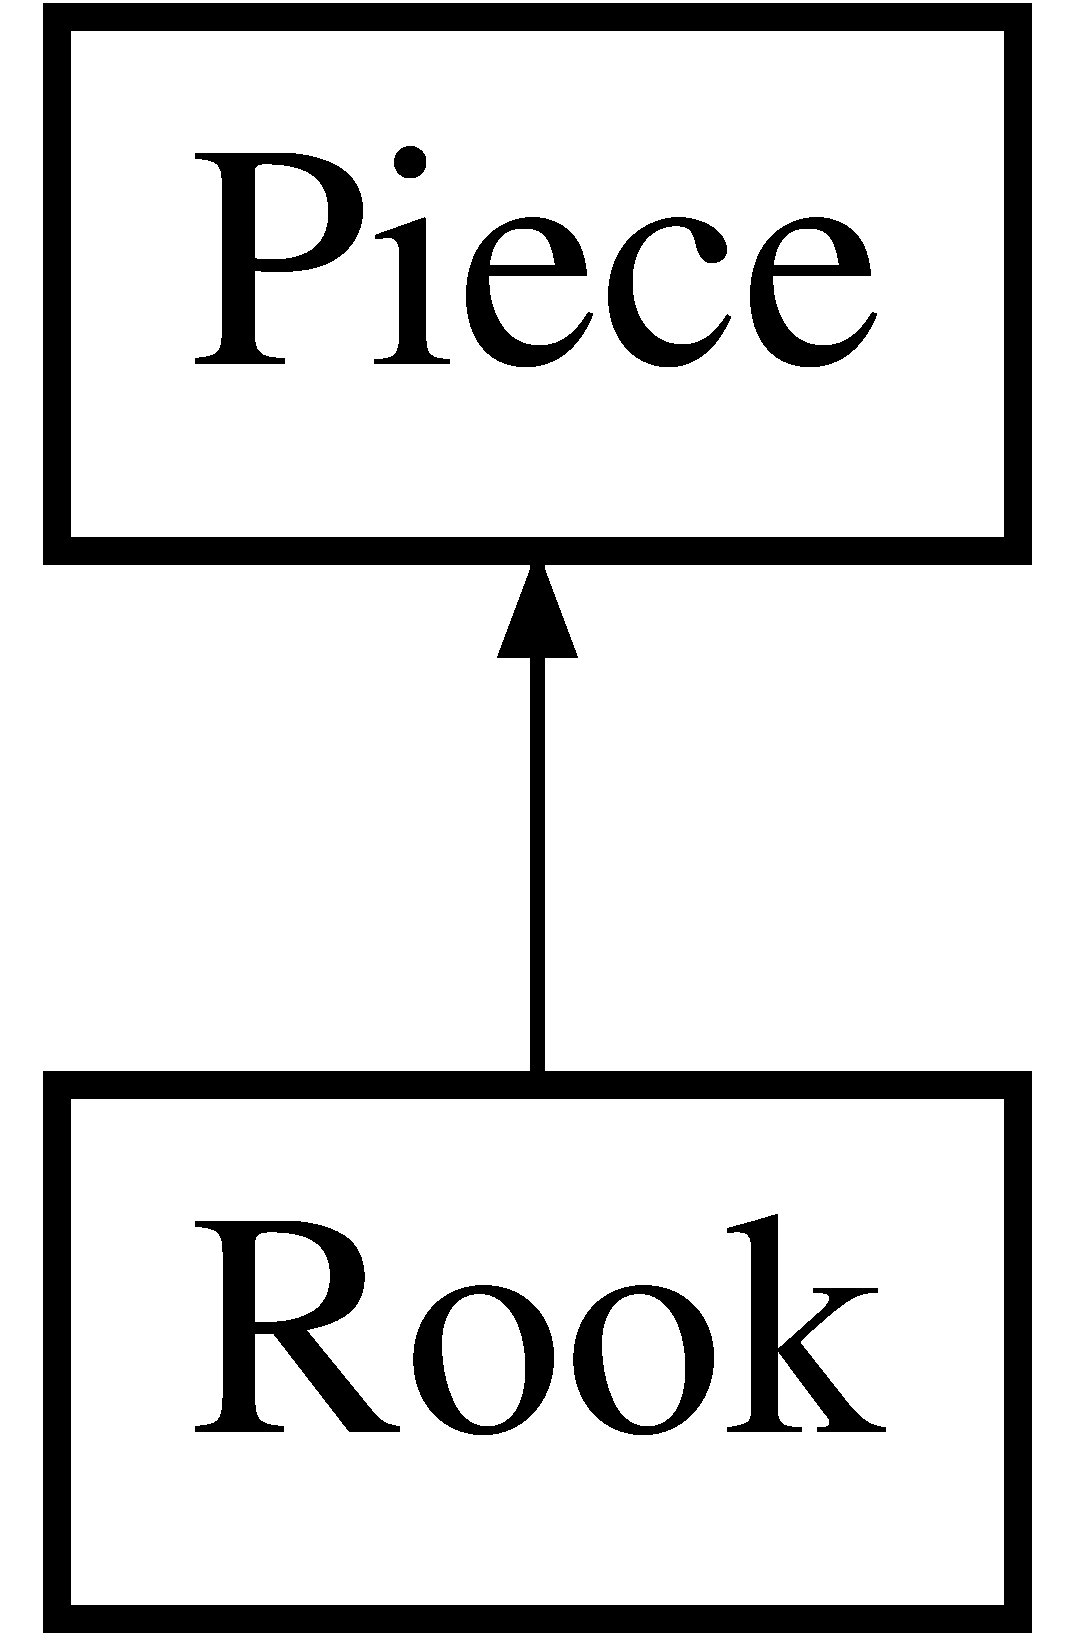
\includegraphics[height=2.000000cm]{class_rook}
\end{center}
\end{figure}
\subsection*{Public Member Functions}
\begin{DoxyCompactItemize}
\item 
\hyperlink{class_rook_a4ee96c73ff3fe981c6b14bb8a60c2a4b}{Rook} (boolean color, int x\+Coord, int y\+Coord)
\item 
boolean \hyperlink{class_rook_a1a6ddf128b86c04e92acae4758b3f10c}{is\+Valid\+Move} (\hyperlink{class_board}{Board} board, int to\+X, int to\+Y)
\item 
boolean \hyperlink{class_rook_a4b521299b8de1bde72c9633cbe91746f}{piece\+In\+Way\+Straight} (\hyperlink{class_board}{Board} board, int to\+X, int to\+Y)
\end{DoxyCompactItemize}
\subsection*{Additional Inherited Members}


\subsection{Constructor \& Destructor Documentation}
\hypertarget{class_rook_a4ee96c73ff3fe981c6b14bb8a60c2a4b}{}\index{Rook@{Rook}!Rook@{Rook}}
\index{Rook@{Rook}!Rook@{Rook}}
\subsubsection[{Rook}]{\setlength{\rightskip}{0pt plus 5cm}Rook.\+Rook (
\begin{DoxyParamCaption}
\item[{boolean}]{color, }
\item[{int}]{x\+Coord, }
\item[{int}]{y\+Coord}
\end{DoxyParamCaption}
)}\label{class_rook_a4ee96c73ff3fe981c6b14bb8a60c2a4b}
\hyperlink{class_rook}{Rook} Constructor 
\begin{DoxyParams}{Parameters}
{\em color} & \\
\hline
{\em x\+Coord} & \\
\hline
{\em y\+Coord} & \\
\hline
\end{DoxyParams}


\subsection{Member Function Documentation}
\hypertarget{class_rook_a1a6ddf128b86c04e92acae4758b3f10c}{}\index{Rook@{Rook}!is\+Valid\+Move@{is\+Valid\+Move}}
\index{is\+Valid\+Move@{is\+Valid\+Move}!Rook@{Rook}}
\subsubsection[{is\+Valid\+Move}]{\setlength{\rightskip}{0pt plus 5cm}boolean Rook.\+is\+Valid\+Move (
\begin{DoxyParamCaption}
\item[{{\bf Board}}]{board, }
\item[{int}]{to\+X, }
\item[{int}]{to\+Y}
\end{DoxyParamCaption}
)}\label{class_rook_a1a6ddf128b86c04e92acae4758b3f10c}
Check if Valid Move 
\begin{DoxyParams}{Parameters}
{\em board} & \\
\hline
{\em to\+X} & \\
\hline
{\em to\+Y} & \\
\hline
\end{DoxyParams}
\begin{DoxyReturn}{Returns}

\end{DoxyReturn}
\hypertarget{class_rook_a4b521299b8de1bde72c9633cbe91746f}{}\index{Rook@{Rook}!piece\+In\+Way\+Straight@{piece\+In\+Way\+Straight}}
\index{piece\+In\+Way\+Straight@{piece\+In\+Way\+Straight}!Rook@{Rook}}
\subsubsection[{piece\+In\+Way\+Straight}]{\setlength{\rightskip}{0pt plus 5cm}boolean Rook.\+piece\+In\+Way\+Straight (
\begin{DoxyParamCaption}
\item[{{\bf Board}}]{board, }
\item[{int}]{to\+X, }
\item[{int}]{to\+Y}
\end{DoxyParamCaption}
)}\label{class_rook_a4b521299b8de1bde72c9633cbe91746f}
Check if straight move is valid 
\begin{DoxyParams}{Parameters}
{\em board} & \\
\hline
{\em to\+X} & \\
\hline
{\em to\+Y} & \\
\hline
\end{DoxyParams}
\begin{DoxyReturn}{Returns}

\end{DoxyReturn}


The documentation for this class was generated from the following file\+:\begin{DoxyCompactItemize}
\item 
src/Rook.\+java\end{DoxyCompactItemize}

\hypertarget{class_rook_test}{}\section{Rook\+Test Class Reference}
\label{class_rook_test}\index{Rook\+Test@{Rook\+Test}}
\subsection*{Public Member Functions}
\begin{DoxyCompactItemize}
\item 
\hypertarget{class_rook_test_a2d1311a187a6d0afdd96e4225f9342c2}{}void {\bfseries test\+Simple\+Move} ()  throws Exception \label{class_rook_test_a2d1311a187a6d0afdd96e4225f9342c2}

\item 
\hypertarget{class_rook_test_a6bbef09ae19196d68873ddb1a72c1d8b}{}void {\bfseries test\+Capture} ()  throws Exception \label{class_rook_test_a6bbef09ae19196d68873ddb1a72c1d8b}

\item 
\hypertarget{class_rook_test_a394de28faebf871ee55a14c2145071f3}{}void {\bfseries test\+Piece\+In\+Way} ()  throws Exception \label{class_rook_test_a394de28faebf871ee55a14c2145071f3}

\item 
\hypertarget{class_rook_test_a6bad72f1735a97416a70f63fa308a481}{}void {\bfseries test\+Illegal\+Move} ()  throws Exception \label{class_rook_test_a6bad72f1735a97416a70f63fa308a481}

\end{DoxyCompactItemize}


The documentation for this class was generated from the following file\+:\begin{DoxyCompactItemize}
\item 
Test/Rook\+Test.\+java\end{DoxyCompactItemize}

%--- End generated contents ---

% Index
\backmatter
\newpage
\phantomsection
\clearemptydoublepage
\addcontentsline{toc}{chapter}{Index}
\printindex

\end{document}
